%
% packages & config
%

\documentclass[utf8,english]{gradu3}

\usepackage{graphicx}
\usepackage{float}
\usepackage{csquotes}
\usepackage{amsmath,amssymb,amsthm}
\usepackage{biblatex}
\usepackage[bookmarksopen,bookmarksnumbered,linktocpage]{hyperref}
\usepackage{algorithmicx}
\usepackage{algpseudocode}

\usepackage{tikz}
\usetikzlibrary{arrows.meta}
\tikzset{>=latex}
\usetikzlibrary{3d}
\usetikzlibrary{calc}

\usepackage{pgfplots}
\pgfplotsset{compat=1.9}

% restore the default LaTeX font for \mathcal
% (gradu3.cls contains font config that makes it unreadable)
\DeclareMathAlphabet{\mathcal}{OMS}{cmsy}{m}{n}

% matrices with customizable stretch
% as per https://tex.stackexchange.com/questions/14071/how-can-i-increase-the-line-spacing-in-a-matrix
\makeatletter
\renewcommand*\env@matrix[1][\arraystretch]{%
  \edef\arraystretch{#1}%
  \hskip -\arraycolsep
  \let\@ifnextchar\new@ifnextchar
  \array{*\c@MaxMatrixCols c}}
\makeatother

%
% metadata
%

\addbibresource{sources.bib}

\title{Discrete Exterior Calculus and Exact Controllability for Time-Harmonic Acoustic Wave Simulation}
\translatedtitle{Diskreetti ulkoinen laskenta ja kontrollimenetelmä aikaharmonisessa akustiikka\-simulaatiossa}
\author{Mikael Myyrä}
\contactinformation{\texttt{mikael.b.myyra@jyu.fi}}
\supervisor{Sanna Mönkölä, Tuomo Rossi, Jonni Lohi, Tytti Saksa}
\studyline{Mathematical modelling in science and decision analytics}
\abstract{
Discrete exterior calculus (DEC) is a
discretization method for differential equations
which preserves important geometric properties of physical models
and produces computationally efficient algorithms.
We investigate ways to improve the performance of DEC
in the context of time-periodic solutions
to acoustic wave scattering problems
by using operators purpose-built for harmonic problems
and an optimization approach based on exact controllability.
The harmonic operators are found to improve accuracy significantly,
while the controllability method is found to be a good choice only
in problems with highly nonconvex geometry.
Computation mesh quality is identified as a key issue
in the accuracy and stability of these methods.
}
\tiivistelma{
Diskreetti ulkoinen laskenta (engl, discrete exterior calculus, DEC)
on differentiaaliyhtälöiden ratkaisemiseen soveltuva diskretointimenetelmä,
jo\-ka säilyttää tiettyjä fysikaalisten mallien geometrisia ominaisuuksia
ja tuottaa laskennallisesti tehokkaita algoritmeja.
Tutkimme keinoja tehostaa DEC:n suorituskykyä
aikaharmonisten ratkaisujen selvittämisessä
akustisten aaltojen sirontaa kuvaaville tehtäville.
Käytämme harmonisille malleille suunniteltuja operaattoreita
ja eksaktiin kontrolloitavuuteen perustuvaa optimointimenetelmää.
Kokeiluissamme harmoniset operaattorit lisäävät menetelmän tark\-kuutta huomattavasti,
kun taas kontrollimenetelmä osoittautuu hyväksi valinnaksi vain teh\-tävissä,
joiden geometria on huomattavan epäkonveksia.
Laskentaverkon laadulla on suuri mer\-kitys
tutkittujen menetelmien tarkkuudessa ja stabiilisuudessa.
TODO: käytämme -> käytetään ym.
}
\keywords{
discrete exterior calculus,
exact controllability,
time-harmonic,
acoustics,
simulation
}
\avainsanat{
diskreetti ulkoinen laskenta,
kontrollimenetelmä,
aikaharmoninen,
akustiikka,
simulointi
}

%
% begin document
%

\begin{document}

% table of contents generates slightly overfull hboxes for some reason,
% suppress those errors with a bit of fuzz
\hfuzz=1.5pt
\maketitle
\mainmatter
\hfuzz=0pt


\chapter{Introduction}

Discrete exterior calculus (DEC),
developed by \textcite{desbrun_discrete_2005}
with roots leading up to the finite-difference time domain (FDTD)
method of \textcite{yee_numerical_1966}
and the work of Bossavit (TODO refs),
is a discretization method for differential equations
based on the exterior calculus of differential forms.
It is a \textit{mimetic} discretization method,
meaning it preserves certain physically important geometric properties
of the continuous model exactly \parencite{bochev_principles_2006}.
It also provides an efficient explicit timestepping procedure
requiring no solution of linear systems.

DEC has been previously applied to simulations of e.g. electromagnetics
\parencite{rabina_efficient_2015, monkola_discrete_2022},
Darcy flow \parencite{hirani_numerical_2015},
quantum mechanics (TODO: ref: Räbinä, Kivioja, Rossi)
and fluid dynamics \parencite{nitschke_discrete_2017}.
Recently, it has been used to develop a theory 
of general classes of wave propagation problems
in \parencite{rabina_generalized_2018} and \parencite{rossi_systematisation_2021}.

We apply DEC to the propagation and scattering of acoustic waves.
In addition to the baseline DEC, we implement the optimized operators
for harmonic simulations introduced by \textcite{rabina_numerical_2014}
in the context of electromagnetics.
We also investigate ways to use DEC to obtain time-periodic solutions to scattering problems.
A simple asymptotic iteration procedure is compared with an optimization approach
based on the idea of exact controllability developed by \textcite{lions_exact_1988}
and applied to the computation of time-periodic solutions by
\textcite{bristeau_controllability_1998}.
This method has been previously applied to e.g.
electromagnetics \parencite{rabina_numerical_2014},
elastodynamics \parencite{monkola_time-harmonic_2008},
and acoustics \parencite{kahkonen_solution_2011}.
The method can be used with any forward-in-time solver,
such as finite element or finite difference solvers.
\parencite{rabina_numerical_2014} is an example of usage specifically with DEC.

TODO: maybe something about implementation here

TODO: check parentheses in citations

This thesis is structured as an extended version of the article (TODO)
(provided as appendix TODO)
with an emphasis on explaining the mathematical theory of the methods used.
An effort is made to provide intuitions rather than rigorous mathematical definitions,
intended as a suitable starting point for students unfamiliar with the topic
but with some experience in mathematics.
Chapters \ref{cha:dec} and \ref{cha:controllability} cover the theory of discrete exterior calculus
and the exact controllability method, respectively.
The simulation model used in our numerical experiments is defined in chapter \ref{cha:model},
and the experiments themselves are discussed in chapter \ref{cha:experiments}.


\chapter{Discrete exterior calculus}\label{cha:dec}

The mathematical theory underlying discrete exterior calculs
is the exterior calculus of differential forms,
which provides a way to express differential equations
in a way that lends itself to a straightforward and systematic
method of discretization where continuous operators
have direct discrete analogues.
This chapter gives a brief introduction to exterior calculus
followed by a description of the mesh- and cochain-based discretization of DEC.
The reader is assumed to be familiar with linear algebra and vector calculus.


\section{Differential forms and the continuous exterior calculus}

This section is meant as a somewhat informal and intuitive introduction
to differential forms, summarizing relevant sections of
\parencite{blair_perot_differential_2014} and \parencite{crane_digital_2013}.
For a more formal and comprehensive approach to the topic,
see a textbook on differential geometry such as \parencite{lee_introduction_2012}
or \parencite{abraham_manifolds_2012}.

TODO: rephrase this to emphasize practicality

TODO: capitalize Section, Chapter, Figure etc.


\subsection{Differential forms}

Notationally, a differential form looks like an \textit{integrand},
e.g. the $dx$ in $\int dx$ or the $5\,dx\,dy$ in $\iint 5\,dx\,dy$.
Indeed, the things we integrate are all technically differential forms.
However, this seems rather abstract.
Are these objects meaningful outside of integration,
and if so, what do they do?
This section looks at differential forms as functions,
taking inspiration from \parencite{crane_digital_2013}.

Differential forms are in many ways analogous to vectors.
To illustrate the similarities and differences,
consider the dot product operation
for two vectors in linear algebra.
Expressed in matrix form, the dot product between vectors
$\mathbf{a} = (a_1, \dots, a_n)^T$ and $\mathbf{b} = (b_1, \dots, b_n)^T$
is

\[
  \mathbf{a} \cdot \mathbf{b} = \mathbf{a}^T \mathbf{b}
  = \begin{bmatrix}
    a_1 & \dots & a_n
  \end{bmatrix}
  \begin{bmatrix}
    b_1 \\ \vdots \\ b_n
  \end{bmatrix}.
\]

The dot product measures the length of $\mathbf{b}$ in the direction of $\mathbf{a}$,
and to do this, $\mathbf{a}$ is transposed into a \textit{row vector}.
This row vector can be thought of as a function
that takes a vector and measures it along $\mathbf{a}$,

\[
  \alpha(\mathbf{b}) = \mathbf{a}^T \mathbf{b}.
\]

A linear function that takes a vector and produces a scalar like this
is called a \textit{covector}.

We can also measure higher-dimensional quantities.
A 2-covector is a function that takes two vectors,
which define a parallelogram,
and computes the area of this parallelogram
when projected onto a plane.
Similarly, 3-covectors measure the volumes of parallelepipeds
defined by three vectors, and so on for higher dimensions.
Additionally, we can define 0-covectors
as objects that take zero vectors as input and return a measurement,
making them equivalent to scalars.

For covectors of dimension 2 and above, we also need to consider
the notion of \textit{signed} areas and volumes.
Much like how the vector cross product flips its direction
depending on whether its arguments come in clockwise or counterclockwise order,
a covectors's output will change its sign
if any two of its arguments are exchanged.
The sign is a measurement of the given volume's \textit{orientation}:
clockwise or counterclockwise for 2D areas,
right-handed or left-handed basis for 3D volumes, etc.
This is why covectors are formally defined as \textit{antisymmetric tensors}
-- they're multilinear functions on vectors (i.e. tensors)
which change sign when arguments are exchanged (i.e. they are antisymmetric).

A differential $k$-form is a \textit{field} of $k$-covectors,
i.e. a function that associates a $k$-covector with every point in space.
Somewhat confusingly, the term $k$-form is also commonly used to
refer to individual $k$-covectors;
a terminology we will adopt from here on.
$k$-form in this thesis will refer to either a $k$-covector
or a field of them depending on context.


\subsection{Proxy vectors}

There is a natural one-to-one correspondence between row and column vectors,
expressed in the transpose operator.
An analogous one-to-one correspondence also exists between 1-forms and vectors.
The operators realizing this correspondence are called
\textit{sharp} $\sharp$ and \textit{flat} $\flat$.
Sharp turns a 1-form into the corresponding vector,
and flat does the reverse.
In other words, given a 1-form $\alpha$,
$v = \alpha^{\sharp}$ is a vector and $v^{\flat} = \alpha$.

We call $v$ a \textit{vector proxy} of $\alpha$.
When performing exterior calculus computations,
the inputs and results are typically interpreted
and visualized as their vector proxies.


\subsection{Basis forms}

Like vectors, differential forms also form a vector space,
meaning they can be expressed as linear combinations of basis vectors.
In $\mathbb{R}^3$, with axes labeled $x$, $y$, and $z$,
the corresponding basis 1-forms are called $dx$, $dy$, and $dz$.

Higher-dimensional forms also have this vector space structure,
but defining a basis for them is not quite as straightforward.
The issue is that $n$-forms measure $n$-dimensional geometric objects
which require $n$ different vectors to define.
Thus, to define an $n$-form we need a formal way to combine
measurements in $n$ different directions.
The operator which does this is called the \textit{exterior product}.


\subsection{Exterior product}

You may recall from linear algebra that the signed area of a parallelogram
defined by two vectors $u,v$ in $\mathbb{R}^3$ is computed
by the cross product $u \times v$.
Similarly, the volume of a parallelepiped defined by three vectors $u,v,w$
is computed by the triple product $(u \times v) \cdot w$,
and in general the volume spanned by $n$ vectors $v_1, \dots, v_n$
is the determinant
\[
  \det \begin{bmatrix}
    v_1, \dots, v_n
  \end{bmatrix}.
\]

The analogous operation for differential forms is called the
\textit{exterior product} or \textit{wedge product} $\wedge$,
which takes a $k$-form $\alpha$ and a $j$-form $\beta$
and produces a $(k+j)$-form which measures volumes spanned by
$\alpha$ and $\beta$ combined.
For instance, if $\alpha$ and $\beta$ are both 1-forms,
$\alpha \wedge \beta$ is a 2-form which measures parallelograms
in the plane spanned by $\alpha$ and $\beta$.

Depending on the dimension of forms being multiplied,
the wedge product's sign may change
when the order of its arguments is flipped. Specifically,
\begin{equation}\label{eq:wedge_antisymmetry}
  \alpha \wedge \beta = (-1)^{kj} \beta \wedge \alpha.
\end{equation}
Additionally, the wedge product is associative, meaning
\begin{equation}
  (\alpha \wedge \beta) \wedge \gamma = \alpha \wedge (\beta \wedge \gamma).
\end{equation}

These three properties (addition of dimensions, antisymmetry, and associativity)
are enough to define the wedge product abstractly in all dimensions.
In practice, what this operation looks like depends on the dimension of its operands
in a way that mirrors the vector operations measuring volumes.
The wedge product of two 1-forms in 3D space
is equivalent to the cross product on the vector proxies of the forms,
and the wedge product of three 1-forms (really a 2-form and a 1-form)
is equivalent to the triple product on the vector proxies.
Additionally, since a 0-form is just a scalar,
the wedge product of a 0-form with anything is a scalar multiplication.

To give a specific example, consider two 1-forms $\alpha, \beta$ in $\mathbb{R}^3$.
The wedge product $\alpha \wedge \beta$
is equivalent to $\star(\alpha^{\sharp} \times \beta^{\sharp})^{\flat}$
(where the star symbol, not important yet but included for accuracy's sake,
is the \textit{Hodge star} operator covered later in section \ref{sec:hodge}).
The resulting 2-form is applied to two vectors $u,v$ as
\[
  \alpha \wedge \beta (u,v) = \alpha(u)\beta(v) - \alpha(v)\beta(u),
\]
and the resulting value is the area of the parallelogram
defined by the projections of $u$ and $v$
onto a plane whose basis vectors are $\alpha^{\sharp}$ and $\beta^{\sharp}$.

The 1-form wedge product can be visualized as combining two vectors
into a single oriented parallelogram,
or in a sense, two basis elements of a line
into a basis element of a plane.
Similarly, further wedge products add on more basis elements,
producing higher-dimensional oriented volumes.
This is illustrated in figure \ref{fig:wedge}.

\begin{figure}[h]
  \centering
  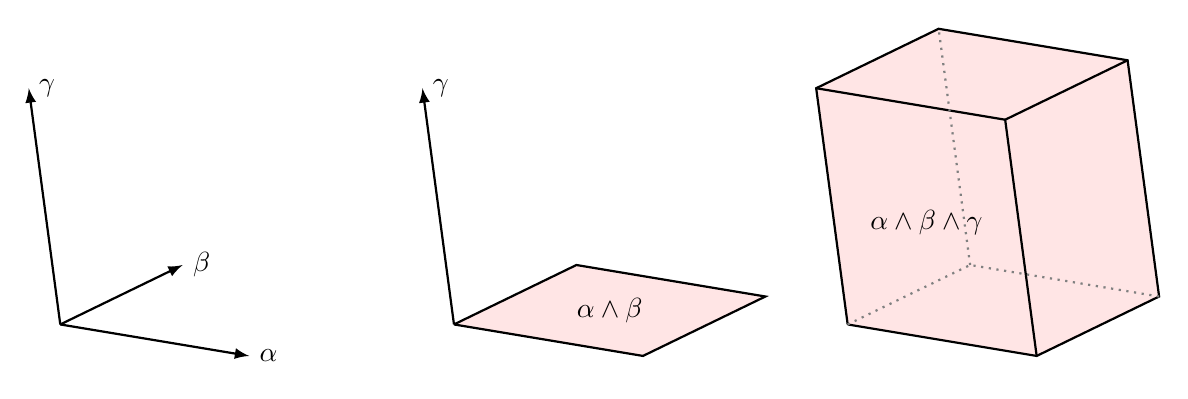
\begin{tikzpicture}[scale=2, thick]
    \coordinate (x) at (1.2, -0.2, 0);
    \coordinate (z) at (0.2, -0.2, -1.5);
    \coordinate (y) at (-0.2, 1.5, 0);
    \draw[->] (0,0,0) -- (x);
    \draw[->] (0,0,0) -- (z);
    \draw[->] (0,0,0) -- (y);
    \node[anchor=west] at (x) {$\alpha$};
    \node[anchor=west] at (z) {$\beta$};
    \node[anchor=west] at (y) {$\gamma$};

    \begin{scope}[xshift=2.5cm]
      \coordinate (x) at (1.2, -0.2, 0);
      \coordinate (z) at (0.2, -0.2, -1.5);
      \coordinate (y) at (-0.2, 1.5, 0);
      \draw[fill=red!10] (0,0,0) -- (x) -- ($(x) + (z)$) -- (z) -- (0,0,0);
      \draw[->] (0,0,0) -- (y);
      \node at ($0.5*(x) + 0.5*(z)$) {$\alpha \wedge \beta$};
      \node[anchor=west] at (y) {$\gamma$};
    \end{scope}

    \begin{scope}[xshift=5cm]
      \coordinate (x) at (1.2, -0.2, 0);
      \coordinate (z) at (0.2, -0.2, -1.5);
      \coordinate (y) at (-0.2, 1.5, 0);
      \fill[fill=red!10] (0,0,0) -- (x) -- ($(x) + (z)$) -- ($(x) + (y) + (z)$) -- ($(y) + (z)$) -- (y) -- (0,0,0);
      \draw (0,0,0) -- (x) -- ($(x) + (z)$) -- ($(x) + (y) + (z)$) -- ($(y) + (z)$) -- (y) -- (0,0,0);
      \draw (x) -- ($(x) + (y)$) -- ($(x) + (y) + (z)$);
      \draw (y) -- ($(x) + (y)$);
      \draw[gray,dotted] (0,0,0) -- (z) -- ($(x) + (z)$);
      \draw[gray,dotted] (z) -- ($(z) + (y)$);
      \node at ($0.5*(x) + 0.5*(y)$) {$\alpha \wedge \beta \wedge \gamma$};
    \end{scope}
  \end{tikzpicture}
  \caption{Exterior products of 1-forms visualized as volumes.}
  \label{fig:wedge}
\end{figure}

Thinking about an $n$-form as an oriented piece
of an $n$-dimensional subspace like this is an intuition
which will be useful in understanding the operations of exterior calculus.

Naturally, the dimension of a form cannot exceed that of the space it's embedded in.
Thus, the wedge product in $n$-dimensional space
is only defined for operands whose dimensions sum to $n$ or less.

A consequence of the wedge product being defined to measure volumes
(algebraically, a consequence of the antisymmetry equation \eqref{eq:wedge_antisymmetry})
is that the wedge product of a $k$-form with itself is zero when $k$ is odd;
\[
  \alpha \wedge \beta = -\beta \wedge \alpha
  \implies \alpha \wedge \alpha = 0.
\]
This is because, intuitively, two parallel vectors
form a parallelogram with zero area,
and in general a linearly dependent set of vectors
forms a degenerate volume.

On the other hand, when $k$ is even (including zero),
antisymmetry does not apply and $\alpha \wedge \alpha$ behaves like a dot product.
For 0-forms, whose wedge product is scalar multiplication,
this means $\alpha \wedge \alpha = \alpha^2$.
For higher-dimensional forms this only begins to apply in four dimensions,
where 2-forms can be multiplied.

TODO: the above paragraph is wrong

Equipped with the exterior product,
we can define a basis for higher-dimensional forms.


\subsection{Higher-dimensional basis forms}\label{sec:basis_higher}

Basis forms of dimension 2 and above
are defined in terms of basis 1-forms and the exterior product.

In three dimensions, there are obviously three basis 1-forms.
The basis of 2-forms also has three elements,
or in other words, there are three linearly independent basis planes.
This number can be deduced algebraically
by taking the wedge product of all possible pairs of basis 1-forms
and eliminating ones that are either zero or a multiple of another.
A more intuitive geometric reasoning is that 
a plane in three dimensions is uniquely identified by its normal vector;
therefore the space of all planes has the same dimension as the space of all vectors.

There is only one three-dimensional subspace of three-dimensional space,
and thus only one basis 3-form.
This is true for any $n$:
there is only one basis $n$-form in $n$-dimensional space.
This form is called the \textit{volume form} of the space,
and it behaves like a scalar in computations.
Table \ref{tab:basis_3d} lists the basis forms in $\mathbb{R}^3$.

\begin{table}[h]
  \begin{tabular}{c | l}
    $n$ & basis $n$-forms \\
    \hline
    0 & 1 \\
    1 & $dx$,\, $dy$,\, $dz$ \\
    2 & $dx \wedge dy$,\, $dy \wedge dz$,\, $dz \wedge dx$ \\
    3 & $dx \wedge dy \wedge dz$ \\
  \end{tabular}
  \caption{Basis forms in $\mathbb{R}^3$.}
  \label{tab:basis_3d}
\end{table}

In two dimensions things are somewhat simpler,
as there is only one plane, and the 2-form is the volume form.
Table \ref{tab:basis_2d} lists the basis forms in $\mathbb{R}^2$.

\begin{table}[h]
  \begin{tabular}{c | l}
    $n$ & basis $n$-forms \\
    \hline
    0 & 1 \\
    1 & $dx$,\, $dy$ \\
    2 & $dx \wedge dy$ \\
  \end{tabular}
  \caption{Basis forms in $\mathbb{R}^2$.}
  \label{tab:basis_2d}
\end{table}

\subsection{Hodge star}\label{sec:hodge}

Consider the idea mentioned in section \ref{sec:basis_higher}
that a plane in three dimensions is uniquely identified by its normal vector.
This is one manifestation of the general fact that a linear subspace
is uniquely identified by its orthogonal complement.
In the context of differential forms,
an analogous statement is that there is an equal number
of basis $k$-forms and $(n-k)$-forms in $n$-dimensional space
and the map from a $k$-form to its orthogonal $(n-k)$-form
is an isomorphism.

The isomorphism taking a $k$-form to the orthogonal $(n-k)$-form
with the same magnitude is an important operator
called the \textit{Hodge star} $\star$.
It is a linear operator whose effect on the $\mathbb{R}^3$ basis forms
is as follows:

\begin{align*}
  \star 1 &= dx \wedge dy \wedge dz \\
  \star dx &= dy \wedge dz \\
  \star dy &= dz \wedge dx \\
  \star dz &= dx \wedge dy \\
  \star (dx \wedge dy) &= dz \\
  \star (dy \wedge dz) &= dx \\
  \star (dz \wedge dx) &= dy \\
  \star (dx \wedge dy \wedge dz) &= 1 \\
\end{align*}

Applying the star twice amounts to doing nothing at all,
$\star\star\alpha = \alpha$.

In $\mathbb{R}^2$ this is complicated slightly by the fact that
the orthogonal complement of a line is also a line,
and the Hodge star on 1-forms amounts to a 90 degree rotation.
Hence, for 1-forms in $\mathbb{R}^2$, a star twice is a 180 degree rotation,
$\star\star\alpha = -\alpha$.
In general, for $k$-forms in $n$-dimensional space,
\[
  \star\star\alpha = (-1)^{k(n-k)}\alpha.
\]

The effect of the Hodge star on the $\mathbb{R}^2$ basis forms is
\begin{align*}
  \star 1 &= dx \wedge dy \\
  \star dx &= dy \\
  \star dy &= -dx \\
  \star (dx \wedge dy) &= 1 \\
\end{align*}


\subsection{Exterior derivative}\label{sec:ext_der}

The final operations we need to define the \textit{calculus} part of exterior calculus
are differentiation and integration.
Integration is exactly the procedure familiar from multivariate calculus
(differential forms are integrands, after all).
1-forms can be integrated over curves, 2-forms over surfaces,
3-forms over volumes, and so on.
Differentiation is performed by the \textit{exterior derivative} $\mathbf{d}$,
which, like the exterior product,
is equivalent to several different vector operators
depending on the dimension of its operand.

A common property of the exterior derivative regardless of dimension
is that it increases the dimension of its operand by one.
In other words, the exterior derivative of a $k$-form $\alpha$ is a $(k+1)$-form.
This, along with the \textit{product rule}
\[
  \mathbf{d}(\alpha \wedge \beta)
  = \mathbf{d}\alpha \wedge \beta + (-1)^k \beta \wedge \mathbf{d}\alpha,
\]
the property $\mathbf{d} \circ \mathbf{d} = 0$,
and the definition of $\mathbf{d}$ for 0-forms,
can be used to recursively define the exterior derivative for all dimensions,
but as with the wedge product, the formal definition is very abstract.
An intuitive explanation of why $\mathbf{d}$ is defined this way
is outside the scope of this thesis,
but a reasoning based on the \textit{differential of a manifold}
is given in \cite{crane_digital_2013}.
For our purposes it will suffice to cover the equivalent vector proxy operations
for each dimension of $\mathbf{d}$.

A 0-form $f$ is a scalar function.
Its exterior derivative is the gradient, also known as the differential,
\[
  \mathbf{d}f = \nabla f = df.
\]
Omitting conversions with $\sharp$, $\flat$ and $\star$ for clarity,
the exterior derivative of a 1-form $\alpha$ corresponds to the
\textit{curl} of the vector proxy,
\[
  \mathbf{d}\alpha \eqsim \nabla \times \alpha.
\]
The exterior derivative of the volume form is not defined
(as it would produce a form of higher dimension than the space),
so in two dimensions this is the final $\mathbf{d}$.
In three dimensions, the exterior derivative of a 2-form $\beta$
is the \textit{divergence} of the (perpendicular) vector proxy,
\[
  \mathbf{d}\beta \eqsim \nabla \cdot \beta.
\]

These relationships give rise to \textit{Stokes' theorem},
which states that for a $k$-dimensional domain $\Omega$
with boundary $\partial \Omega$ and a $(k-1)$-form $\alpha$,

\begin{equation}\label{eq:stokes_theorem}
  \int_{\Omega} \mathbf{d}\alpha = \int_{\partial\Omega} \alpha.
\end{equation}

This theorem encapsulates several vector calculus identities
such as Green's theorem and the divergence theorem.
It is crucial in defining the discrete exterior calculus
and will be covered in more detail in section \ref{sec:disc_ext_der}.

\subsection{Advantages of exterior calculus}

At this point it would be reasonable to ask what the point of
using differential forms instead of vectors is.
If every operation on differential forms has a vector equivalent,
why the additional abstraction?

Indeed, in two- or three-dimensional Euclidean space,
the differential form and vector representations of problems
are largely equivalent and interchangeable.
One of the main purposes of exterior calculus
is the generalization of these concepts to \textit{higher-dimensional}
and \textit{curved} spaces.
Exterior calculus is readily defined for any dimension
and enables the expression of problems on any \textit{manifold}
(generalization of 2D surfaces, 3D volumes etc.),
incorporating the \textit{metric} (measurement of distances between points)
in a systematic way.

In this thesis, we restrict ourselves to Euclidean 2D space
and thus don't make use of these advantages,
but exterior calculus still has something to offer.
Namely, the DEC provides a straightforward way
to discretize any equation expressed in exterior calculus.


\section{Computation mesh}

The discrete spatial structure at the root of the DEC is the \textit{simplicial complex}:
essentially a mesh (in the computer graphics sense)
consisting of triangles in two dimensions,
tetrahedra in three dimensions, or \textit{$k$-simplices} in $k$ dimensions.
We will focus on the two-dimensional case here for illustration.
This section is based on \parencite{desbrun_discrete_2006}.


\subsection{Simplices}

A \textit{$k$-simplex} is the simplest type of $k$-dimensional element
in a polyhedral mesh, defined as
the convex hull of $k + 1$ geometrically distinct points.
In concrete terms, a 0-simplex is a single point,
a 1-simplex is a line segment, a 2-simplex is a triangle,
a 3-simplex is a tetrahedron, and so on.
In the context of a mesh, a 0-simplex is often called a \textit{vertex},
a 1-simplex an \textit{edge}, a 2-simplex a \textit{face},
and a $k$-simplex where $k > 2$ a \textit{volume} or \textit{$k$-volume}.

Every simplex with dimension $k > 0$
has a \textit{boundary} consisting of $(k-1)$-simplices.
For instance, every triangle (2-simplex) is bounded by three line segments (1-simplices),
and every line segment is bounded by two vertices.
Each $(k-1)$-simplex on the boundary of a $k$-simplex $\sigma_k$
is called a \textit{$(k-1)$-face} of $\sigma_k$.

We denote simplices by listing their vertices, e.g. a triangle
$\sigma_2 = \{v_0, v_1, v_2\}$.


\subsection{Simplicial complex}

A simplicial complex $\mathcal{K}$ is a set of simplices satisfying the rules

\begin{itemize}
  \item every face of every simplex in $\mathcal{K}$ is also in $\mathcal{K}$
  \item any two simplices in $\mathcal{K}$ either do not intersect at all
    or share an entire face.
\end{itemize}

In the case of a 2D triangle mesh, this means
that every edge and vertex of every triangle is also part of the complex,
and there are no overlapping triangles
or edges/vertices that aren't part of a triangle's boundary.

A similar complex could be defined without requiring
all its elements to be simplicial.
For instance, a rectilinear grid is a common such structure.
A complex like this is called a \textit{cell complex}
and its $k$-dimensional elements \textit{$k$-cells}.
A simplex is a special case of a cell,
and the concepts of boundary and face apply to all cells.
We will use a simplicial complex in this thesis,
however, non-simplicial cells become relevant in the \textit{dual mesh}
(section \ref{sec:dual_mesh}).


\subsection{Orientation of a simplex}

Much like how differential forms of dimension 2 and higher
have a notion of two distinct orientations,
which manifest themselves in the sign of measured volumes,
simplices with 2 or more vertices also have two possible orientations
depending on the order of the vertices.
For a line segment there are two possible ways to order its two vertices,
for a triangle there are three clockwise and three counterclockwise orderings,
and so on.

As part of the definition of our simplicial complex,
each simplex receives an orientation.
For reasons that will become clear when
we define the discrete exterior derivative in section \ref{sec:disc_ext_der},
every simplex also needs its boundary to match its orientation.
For a counterclockwise oriented triangle, for instance,
this means the boundary line segments must form
a counterclockwise circulation around the triangle.
Since a line segment is often part of two triangles with conflicting orientations,
the defined orientations cannot be consistent with every boundary.

To resolve inconsistent face orientations,
the \textit{boundary operator} $\partial$,
which takes a simplex and returns its faces,
must flip every face that doesn't match the desired orientation.
This is denoted as a multiplication by -1.
For example, the boundary of a counterclockwise oriented triangle $\{v_0, v_1, v_2\}$
with edges $\{v_0, v_1\}$, $\{v_1, v_2\}$, $\{v_0, v_2\}$ is
\[
  \partial \{v_0, v_1, v_2\} = \{v_0, v_1\} + \{v_1, v_2\} - \{v_0, v_2\}.
\]

\begin{figure}[h]
  \centering
  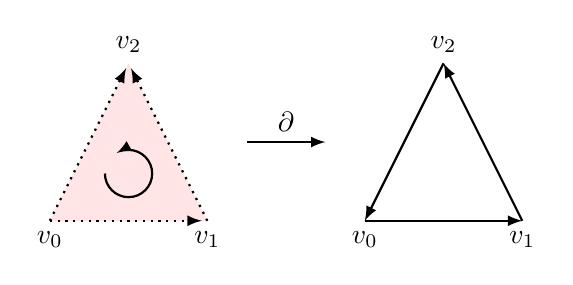
\begin{tikzpicture}
    \fill[fill=red!10] (-1,0) -- (1,0) -- (0,2);
    \draw[thick, dotted, -{>[sep=2pt]}] (-1,0) node[anchor=north]{$v_0$} -- (1,0);
    \draw[thick, dotted, -{>[sep=2pt]}] (1,0) node[anchor=north]{$v_1$} -- (0,2);
    \draw[thick, dotted, -{>[sep=2pt]}] (-1,0) -- (0,2) node[anchor=south]{$v_2$};
    \draw[thick, ->] (-0.3,0.6) arc (-180:120:0.3);

    \draw[thick, ->] (1.5, 1) -- node[anchor=south]{$\partial$} (2.5, 1);

    \draw[thick, ->] (3,0) node[anchor=north]{$v_0$} -- (5,0);
    \draw[thick, ->] (5,0) node[anchor=north]{$v_1$} -- (4,2);
    \draw[thick, ->] (4,2) node[anchor=south]{$v_2$} -- (3,0);
  \end{tikzpicture}
  \caption{
    \label{fig:triangle_boundary}
    Boundary of a triangle with inconsistently oriented faces.
  }
\end{figure}


\subsection{Chains and cochains}\label{sec:chains}

A \textit{$k$-chain} on a simplicial complex $\mathcal{K}$
is a set of real values associated with every $k$-simplex in $\mathcal{K}$.
Denoting the set of all $k$-simplices in $\mathcal{K}$ by $\mathcal{K}^k$
and its cardinality by $|\mathcal{K}^k|$,
a natural represenation for a chain is a $|\mathcal{K}^k|$-dimensional vector.
The space of all $k$-chains $\mathcal{C}_k$ is a vector space,
and the set of all $k$-simplices can be thought of as its basis.

Whereas a chain is analogous to a vector,
a \textit{cochain} is analogous to a differential form:
a linear function that takes a chain and ''measures'' it,
producing a real number.
Formally, cochains exist in the \textit{dual space} $\mathcal{C}_k^*$ of $\mathcal{C}_k$.
A $k$-cochain $\widehat{\alpha} \in \mathcal{C}_k^*$
has one linear operation for each $k$-simplex in $\mathcal{K}$,
matching the dimension of the corresponding $k$-chain $c \in \mathcal{C}_k$,
and the evaluation $\widehat{\alpha}(c)$
behaves like a dot product between vectors.
Thus, a natural way to represent a cochain
is a $|\mathcal{K}^k|$-dimensional \textit{row vector}.

This analogy with differential forms will be useful
when we define discrete forms in the next section.


\section{Discrete differential forms}

Equipped with an oriented simplicial complex,
we can begin to map differential forms and their operations onto it.
This section is based on concepts covered by \parencite{desbrun_discrete_2006},
\parencite{crane_digital_2013}, and \parencite{blair_perot_differential_2014}.


\subsection{Definition of discrete forms}\label{sec:discrete_forms}

Recalling that differential forms can be integrated
over manifolds of matching dimension,
a natural way to map a continuous form to a discrete value on a simplex
is to integrate the form over that simplex.
In other words, given a differential $k$-form $\alpha$
and $k$-simplex $\sigma_k$, we can get a scalar value $\widehat{\alpha}$
associated with $\sigma_k$ by computing the integral

\[
  \widehat{\alpha} = \int_{\sigma_k} \alpha.
\]

This is a line integral over a line segment for 1-forms,
surface integral over a triangle for 2-forms,
volume integral over a tetrahedron for 3-forms, and so on.
Additionally, a 0-form (i.e. a scalar field)
integrated over a 0-simplex (i.e. a single point)
is the value of the form at that point.

Computing this integral for every $k$-simplex in a simplicial complex $\mathcal{K}$
produces a set of values associated with the $k$-simplices,
which can be interpreted as a chain or cochain.
Due to the analogous nature of differential forms and cochains
covered in section \ref{sec:chains},
the most fitting choice of interpretation here is a cochain.
This leads us to the following definition:

A discrete differential $k$-form on an oriented simplicial complex $\mathcal{K}$
is a $k$-cochain obtained by integrating a continuous $k$-form
over every $k$-simplex in $\mathcal{K}$.

The discrete equivalent of a differential form being a cochain,
the discrete versions of the operations of exterior calculus
are operations on cochains.


\subsection{Discrete exterior derivative}\label{sec:disc_ext_der}

Section \ref{sec:ext_der} briefly introduced Stokes' theorem
(equation \ref{eq:stokes_theorem}).
In the domain of a $k$-simplex $\sigma$, it states that
\begin{equation}\label{eq:stokes_simplex}
  \int_{\sigma} \mathbf{d}\alpha = \int_{\partial\sigma} \alpha,
\end{equation}
where $\alpha$ is a $(k-1)$-form.

Writing this in terms of the exterior derivative's
vector analogues covered in section \ref{sec:ext_der}
($\nabla$, $\nabla \times$, and $\nabla \cdot$)
yields several well-known vector calculus identities.

When $k = 1$, equation \ref{eq:stokes_simplex}
is the fundamental theorem of calculus
\begin{equation}\label{eq:fund_theorem_calc}
  \int_{\sigma} \nabla \alpha = \alpha(v_2) - \alpha(v_1)
\end{equation}
where $v_1,v_2$ are the endpoints of the line segment $\sigma$.

When $k = 2$, we get the curl theorem
\begin{equation}\label{eq:curl_theorem}
  \iint_{\sigma} (\nabla \times \alpha) \cdot dA = \int_{\partial\sigma} \alpha \cdot ds,
\end{equation}
which is equivalent to Green's theorem in two-dimensional space.

Finally, when $k = 3$, we get the divergence theorem
\begin{equation}\label{eq:divergence_theorem}
  \iiint_{\sigma} (\nabla \cdot \alpha) \,dV = \iint_{\partial\sigma} \alpha \,dA.
\end{equation}

Stokes' theorem expresses and generalizes the common property between these identities,
that an integral over a $k$-dimensional volume
can be turned into an integral over the volume's
$(k-1)$-dimensional boundary and vice versa.
It is a powerful theorem with many applications.
For the use case of discrete exterior calculus,
it can be used as the \textit{definition} of
the discrete exterior derivative.
More specifically, we can define the discrete exterior derivative
as the unique operator $\mathbf{d}$ satisfying equation \ref{eq:stokes_simplex}.

To make this concrete, first note that the integrals here
are exactly how cochain elements were defined in section \ref{sec:discrete_forms}.
$\int_{\sigma} \mathbf{d}\alpha$ is an element of a $k$-cochain,
and $\int_{\partial\sigma} \alpha$ is the sum of all $(k-1)$-cochain elements
constituting the boundary of $\sigma$.
In a sense, $\mathbf{d}$ does the opposite of the boundary operator $\partial$
defined in section \ref{sec:discrete_forms}:
whereas $\partial$ takes a simplex and produces the sum of its faces,
$\mathbf{d}$ takes the sum of a simplex's faces and produces the simplex itself.
In more precise terms, $\mathbf{d}$ is the \textit{adjoint} of $\partial$,
also known as the \textit{coboundary operator}.

Given a simplicial complex $\mathcal{K}$,
$\mathbf{d}$ is a linear map from $\mathcal{K}^{k-1}$ to $\mathcal{K}^k$.
Hence, it can be represented as a $|\mathcal{K}^k| \times |\mathcal{K}^{k-1}|$ matrix.
Each row of this matrix corresponds to one $k$-simplex
and represents a signed sum of its faces taking into account relative orientation.
Each column corresponding to a boundary simplex has a coefficient
of 1 or -1 depending on orientation,
and the rest of the coefficients are zeroes.
Graph theorists call this type of matrix an \textit{adjacency matrix}.

Figure \ref{fig:discrete_ext_derivative} illustrates
the discrete exterior derivative on a small simplicial complex.
The subscript on $\mathbf{d}$ denotes the dimension of the input cochain,
and the numbers in the diagrams represent the index of the mesh element in the cochain.
The triangle faces are all oriented counterclockwise.

\begin{figure}[h]
  \centering
  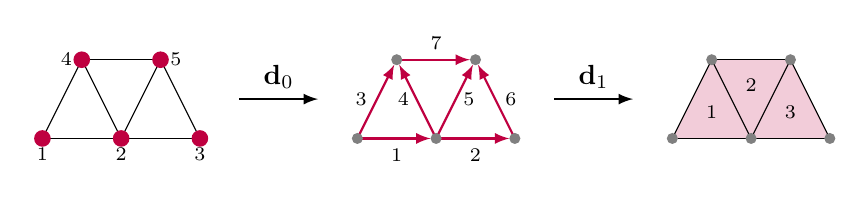
\begin{tikzpicture}
    \draw (0,0) -- (1,0);
    \draw (1,0) -- (2,0);
    \draw (0,0) -- (0.5,1);
    \draw (1,0) -- (0.5,1);
    \draw (1,0) -- (1.5,1);
    \draw (2,0) -- (1.5,1);
    \draw (0.5,1) -- (1.5,1);
    \begin{scope}[font=\scriptsize, fill=purple]
      \fill (0,0) circle (3pt) node[anchor=north]{1};
      \fill (1,0) circle (3pt) node[anchor=north]{2};
      \fill (2,0) circle (3pt) node[anchor=north]{3};
      \fill (0.5,1) circle (3pt) node[anchor=east]{4};
      \fill (1.5,1) circle (3pt) node[anchor=west]{5};
    \end{scope}
    
    \draw[thick, ->] (2.5, 0.5) -- node[anchor=south]{$\mathbf{d}_0$} (3.5,0.5);

    \begin{scope}[xshift=4cm]
      \begin{scope}[thick, font=\scriptsize, draw=purple, -{>[sep=2pt]}]
        \draw (0,0) -- node[below]{1} (1,0);
        \draw (1,0) -- node[below]{2} (2,0);
        \draw (0,0) -- node[left]{3} (0.5,1);
        \draw (1,0) -- node[left=-1pt]{4} (0.5,1);
        \draw (1,0) -- node[right=-1pt]{5} (1.5,1);
        \draw (2,0) -- node[right]{6} (1.5,1);
        \draw (0.5,1) -- node[above]{7} (1.5,1);
      \end{scope}
      \begin{scope}[gray]
        \fill (0,0) circle (2pt);
        \fill (1,0) circle (2pt);
        \fill (2,0) circle (2pt);
        \fill (0.5,1) circle (2pt);
        \fill (1.5,1) circle (2pt);
      \end{scope}
      
      \draw[thick, ->] (2.5, 0.5) -- node[anchor=south]{$\mathbf{d}_1$} (3.5,0.5);
    \end{scope}

    \begin{scope}[xshift=8cm]
      \fill[fill=purple!20] (0,0) -- (2,0) -- (1.5,1) -- (0.5,1);
      \draw (0,0) -- (1,0);
      \draw (1,0) -- (2,0);
      \draw (0,0) -- (0.5,1);
      \draw (1,0) -- (0.5,1);
      \draw (1,0) -- (1.5,1);
      \draw (2,0) -- (1.5,1);
      \draw (0.5,1) -- (1.5,1);
      \begin{scope}[gray]
        \fill (0,0) circle (2pt);
        \fill (1,0) circle (2pt);
        \fill (2,0) circle (2pt);
        \fill (0.5,1) circle (2pt);
        \fill (1.5,1) circle (2pt);
      \end{scope}
      \begin{scope}[font=\scriptsize]
        \node at (0.5,0.33) {1};
        \node at (1,0.67) {2};
        \node at (1.5,0.33) {3};
      \end{scope}
    \end{scope}
  \end{tikzpicture}
  \caption{Discrete exterior derivative visualized on an oriented simplicial complex.}
  \label{fig:discrete_ext_derivative}
\end{figure}

The matrix representations of $\mathbf{d}_0$ and $\mathbf{d}_1$
in figure \ref{fig:discrete_ext_derivative} are

\[
  \mathbf{d}_0 = \begin{bmatrix}[0.8]
    -1 & 1 \\
       & -1 & 1 \\
    -1 & & & 1 \\
       & -1 & & 1 \\
       & -1 & & & 1 \\
       & & -1 & & 1 \\
       & & & -1 & 1 \\
  \end{bmatrix},
  \qquad
  \mathbf{d}_1 = \begin{bmatrix}[0.8]
    1 & & -1 & 1 \\
      & & & -1 & 1 & & -1 \\
      & 1 & & & -1 & 1 \\
  \end{bmatrix}.
\]

A remarkable property of a discrete exterior derivative
defined this way is that it is \textit{exact}.
The value obtained by integrating a form over boundary simplices
and taking the discrete exterior derivative
is exactly the value one would obtain
by first taking the continuous exterior derivative of the same form
and integrating it over the bounded volume.
As a result, use of the discrete exterior derivative in a numerical method
introduces no additional error.
This simplifies the analysis of a method's accuracy
by eliminating one source of error.


\subsection{Dual mesh}\label{sec:dual_mesh}

The continuous Hodge star is an isomorphism
that maps a $k$-form to an orthogonal $(n-k)$-form.
To capture these notions of isomorphism and orthogonality
in the discrete setting, a simplicial complex alone is insufficient.
Some additional geometric structure is needed.

Given a simplicial complex $\mathcal{K}$,
a secondary complex constructed for the purpose of the discrete Hodge star
is called a \textit{dual mesh}, denoted $\mathcal{K}^*$.
When the dual relationship is relevant,
$\mathcal{K}$ is in turn called the \textit{primal mesh}.

The most important property of the dual mesh
is that every $k$-simplex in $\mathcal{K}$
has a corresponding $(n-k)$-cell in $\mathcal{K}^*$.
In two dimensions this means every primal vertex maps to a dual face,
every primal edge maps to a dual edge, and every primal face maps to a dual vertex.
This is illustrated in figure \ref{fig:dual_mesh},
with the purple dotted lines representing the dual mesh.

\begin{figure}[h]
  \centering
  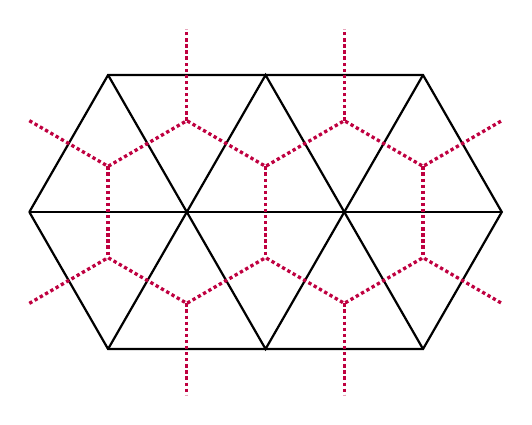
\begin{tikzpicture}[scale=2, thick]
    \draw (0,0) -- (3,0);
    \draw (0,0) -- (0.5,-0.87) -- (2.5,-0.87) -- (3,0) -- (2.5,0.87) -- (0.5,0.87) -- (0,0);
    \draw (0.5,-0.87) -- (1.5,0.87) -- (2.5,-0.87);
    \draw (0.5,0.87) -- (1.5,-0.87) -- (2.5,0.87);

    \begin{scope}[purple, densely dotted, very thick]
      \draw (0,0.58) -- (0.5,0.29) -- (1,0.58) -- (1.5,0.29) -- (2,0.58) -- (2.5,0.29) -- (3,0.58);
      \draw (0,-0.58) -- (0.5,-0.29) -- (1,-0.58) -- (1.5,-0.29) -- (2,-0.58) -- (2.5,-0.29) -- (3,-0.58);
      \draw (0.5,0.29) -- (0.5,-0.29);
      \draw (1.5,0.29) -- (1.5,-0.29);
      \draw (2.5,0.29) -- (2.5,-0.29);
      \draw (1,0.58) -- (1,1.16);
      \draw (2,0.58) -- (2,1.16);
      \draw (1,-0.58) -- (1,-1.16);
      \draw (2,-0.58) -- (2,-1.16);
    \end{scope}
  \end{tikzpicture}
  \caption{A mesh and its dual.}
  \label{fig:dual_mesh}
\end{figure}

Due to this correspondence between elements of the primal and dual meshes,
there is also a correspondence between their boundaries.
Each primal face becomes a dual vertex that is on the boundary
of every dual edge corresponding to the primal face's boundary edges, and so on.
The way this manifests in the adjacency matrix representation of $\mathbf{d}$
is that the $k$-dimensional exterior derivative
on the dual mesh is the \textit{transpose} of the $(n-k-1)$-dimensional
exterior derivative on the primal mesh,
\[
  \mathbf{d}^*_k = \mathbf{d}_{n-k-1}^T.
\]
In a sense, this is the $(n-k)$-dimensional primal coboundary backwards.
This way we only need to compute the exterior derivative matrices
for the primal mesh, and their transposes can be used on the dual.

Notably, a dual mesh is generally not a simplicial one.
For instance, a regular triangular grid in 2D,
such as the one in figure \ref{fig:dual_mesh}, will have hexagonal dual faces.
However, the boundary operator and discrete exterior derivative
are defined in a way that can handle arbitrary polytopes.
The number of faces on a cell merely affects the sparsity pattern
of the matrix $\mathbf{d}$.

A somewhat more challenging property of the dual mesh
are its incomplete faces on the boundary.
For instance, the dual mesh of figure \ref{fig:dual_mesh} has two hexagonal faces
and eight edges pointing outside the primal mesh, connected to nothing at the outer end.
Care must be taken to account for this when defining boundary conditions.
An example of appropriately defined boundary conditions
will be given in section \ref{sec:boundary_conditions}.

There are many possible ways to place the dual elements relative to the primal ones.
In this thesis, \textit{circumcentric} dual cells 
as implemented by the PyDEC software library \parencite{bell_pydec_2012} are used,
meaning the dual vertex of a primal $n$-simplex
is placed at the center of the smallest $n$-ball containing the simplex,
or in other words, at the point that is equidistant from
all vertices of the simplex.
An important property of a dual mesh defined this way is
that primal and dual elements are orthogonal to one another.

\subsection{Discrete Hodge star}\label{sec:discrete_hodge}

The discrete Hodge star is a mapping between $k$-cochains on the primal mesh
and $(n-k)$-cochains on the dual mesh.
By construction of the dual mesh,
this mapping in matrix form is a square $(|\mathcal{K}^k| \times |\mathcal{K}^k|)$-matrix.
For efficient computation, it is desirable for this matrix to be diagonal,
as diagonal matrices are fast to multiply and trivial to invert.

The Hodge star is diagonal when each element of the resulting dual cochain
only depends on its corresponding primal element.
The value of the diagonal elements is based on the idea
that the Hodge star produces a form of equal magnitude.
As we don't generally know the exact form the star will be applied to,
this necessarily involves approximation.

Given a continuous $k$-form $\alpha$, primal $k$-simplex $\sigma$,
and its dual $(n-k)$-cell $\sigma^*$,
a simple approximation for the discrete Hodge star
is obtained by assuming $\alpha$ is constant over $\sigma$ and $\sigma^*$.
Combined with the fact that $\alpha$ and $\star\alpha$ have equal magnitude,
this approximation leads to the idea that the cochains
$\widehat{\alpha} = \int_{\sigma} \alpha$ and $\star\widehat{\alpha} = \int_{\sigma^*} \star\alpha$
should have equal magnitude \textit{per unit of volume},
\[
  \frac{1}{|\sigma|} \widehat{\alpha} = \frac{1}{|\sigma^*|} \star\widehat{\alpha}
  \iff \star\widehat{\alpha} = \frac{|\sigma^*|}{|\sigma|} \widehat{\alpha}.
\]

A discrete Hodge star defined using this approximation
is a square diagonal matrix whose elements are
\begin{equation}
  \star_{ii} = \frac{|\sigma_i^*|}{|\sigma_i|}, \quad i = 1, \dots, |\mathcal{K}^k|.
\end{equation}

A matrix $\star_k$ defined this way takes $k$-cochains from the primal mesh
to $(n-k)$-cochains on the dual mesh.
The $\star^*_{n-k}$ taking $(n-k)$-cochains from the dual mesh back to the primal mesh
is the inverse of this, $\star^*_{n-k} = \star_k^{-1}$.
Knowing this, we only need to compute the Hodge star matrices
in the direction from the primal mesh to the dual, and their inverses
(which are trivial to compute thanks to diagonality)
can be used for the opposite direction.

This approximation, which we call \textit{Yee's Hodge star}
due to its early appearance in \textcite{yee_numerical_1966},
is one of two Hodge star operators used in this thesis.
A different approximation is obtained by assuming spatially harmonic forms
instead of locally constant ones.
The details of this will be covered in section \ref{sec:harmonic_operators}.

Because the discrete exterior derivative is exact,
the Hodge star is the only source of approximation error
in methods based on these two operators.
As such, variants of the discrete Hodge star directly lead to
DEC variants with different accuracy and efficiency characteristics.
Examples of this are the harmonic Hodge star used in this thesis
and the higher order approximations studied by \textcite{lohi_higher_2023}.


\subsection{Interpolating discrete forms}\label{sec:interpolation}

All values in DEC computations are cochains
and thus exist only on elements of a mesh.
However, it is sometimes useful to get the value of a form at a single point.
In this thesis, for instance, we would like to visualize
the 1-form velocity as arrows pointing in the direction of velocity,
but a 1-cochain has no notion of direction.
It only has magnitudes over entire mesh edges.
Thus, direction must be reconstructed by interpolating between multiple nearby edges.
This is accomplished using \textit{Whitney forms},
first introduced by \textcite{whitney_geometric_1957}.
This section gives a short summary of their definition;
see e.g. \parencite{lohi_whitney_2021} for a thorough treatment of the topic.

Whitney forms are defined individually for every simplex
in terms of \textit{barycentric coordinates}:
for a $k$-simplex with vertices $v_0, \dots, v_k$,
any point within the simplex can be expressed as
\[
  \sum_{i=0}^k \lambda_i v_i
\]
where the coefficients $\lambda_i$ are called barycentric coordinates.
If $\sum_{i=0}^k \lambda_i = 1$, these coordinates are called \textit{normalized}.
Equivalently to normalized barycentric coordinates,
the \textit{barycentric function} $\lambda_i$ for a vertex $v_i$
is a piecewise linear function whose value is 1 on $v_i$
and zero on all other vertices.

The Whitney form $\mathcal{W}(v_i)$ associated with a 0-simplex $v_i$
is its barycentric function,
\[
  \mathcal{W}(v_i) = \lambda_i.
\]
For a 1-simplex $\sigma = [v_0,v_1]$, it is
\[
  \mathcal{W}(\sigma) = \lambda_0 d\lambda_1 - \lambda_1 d\lambda_0
\]
or equivalently in vector calculus notation,
\[
  \mathcal{W}(\sigma) = \lambda_0 \nabla\lambda_1 - \lambda_1 \nabla\lambda_0,
\]
and generally for a $k$-simplex $\sigma = [v_0,\dots,v_k]$,
\begin{equation}
  \mathcal{W}(\sigma) = k! \sum_{i=0}^{k} (-1)^i
    \lambda_i d\lambda_1 \wedge \dots \wedge \widehat{d\lambda_i}
    \wedge \dots d\lambda_k
\end{equation}
where $\widehat{\quad}$ denotes that the term is omitted.

Summing these forms across an entire simplicial complex $\mathcal{K}$
produces a piecewise smooth interpolating function called the \textit{Whitney map},
also (somewhat confusingly) denoted $\mathcal{W}$.
Given a $k$-cochain $\hat{\alpha}$ on $\mathcal{K}$ whose element $a_i$
is associated with the $k$-simplex $\sigma_i$,
the $k$-form Whitney map for $\mathcal{K}$ is
\begin{equation}
  \mathcal{W}(\hat{\alpha})
  = \mathcal{W}(\sum_{\sigma_i \in \mathcal{K}^k} a_i\sigma_i)
  = \sum_{\sigma_i \in \mathcal{K}^k} a_i \mathcal{W}(\sigma_i)
\end{equation}

TODO: $\mathcal{W}$ is always the whitney map in the above,
whitney forms are its values. Explain this in this paragraph

Concretely, to evaluate the $k$-form Whitney map for a point $x$,
one would first find the $n$-simplex $x$ lies in
(since all the barycentric functions and hence the Whitney forms
for all simplices outside of it are zero),
where $n$ is the dimension of the working space,
find all the $k$-simplices that are faces of this $n$-simplex,
and sum their respective Whitney forms at $x$.
The use case in this thesis is interpolation of 1-forms in $\mathbb{R}^2$,
in which case one would find the triangle $x$ lies in
with sides $\sigma_0,\sigma_1,\sigma_2$
and associated cochain elements $a_0,a_1,a_2$,
and take the sum
\[
  a_0 (\mathcal{W}(\sigma_0))(x)
  + a_1 (\mathcal{W}(\sigma_1))(x)
  + a_2 (\mathcal{W}(\sigma_2))(x).
\]


\chapter{Model}\label{cha:model}

The physical phenomenon we apply the DEC to
is the propagation and scattering of acoustic waves
in a two-dimensional domain.
This chapter will cover the mathematical models used;
the details of numerical experiments performed and their results
are described in chapter \ref{cha:experiments}.


\section{Vector equations}

We consider waves described by the differential equation

\begin{equation}\label{eq:wave2ndOrd}
  \frac{\partial^2 \phi}{\partial t^2} - c^2 \nabla^2\phi = 0
\end{equation}

where $\phi$ is a velocity potential, $t$ is time
and $c$ is the speed of wave propagation.
This equation is equivalent to the first-order system

\begin{equation}\label{eq:wave1stOrd}
  \begin{cases}
    \frac{\partial p}{\partial t} - c^2\nabla \cdot \mathbf{v} = 0 \\
    \frac{\partial \mathbf{v}}{\partial t} - \nabla p = 0 \\
  \end{cases}
\end{equation}

where $p = \frac{\partial \phi}{\partial t}$ is the scalar-valued acoustic pressure
and $\mathbf{v} = \nabla \phi$ is the vector-valued velocity
of particles perturbed by the wave.

The system \eqref{eq:wave1stOrd} applies within the spatial domain $\Omega$
and the time domain $[0, T]$.


\section{Exterior calculus equations}

The first step to translating the vector system \eqref{eq:wave1stOrd}
to exterior calculus notation is the selection of appropriate differential forms
to represent the variables $p$ and $\mathbf{v}$.
Because a scalar can be represented either by a 0-form or a volume form,
and a vector by a 1-form or $(n-1)$-form,
there are two possible choices for each variable,
both of which can be made equivalent to the vector equations
by the application of Hodge stars when necessary.
The physical properties of a variable can hint at the most appropriate choice,
but one can also begin with 0- and 1-forms
and pick the most convenient representation for the end result.

We begin by representing pressure with the 0-form $p$
and velocity with the 1-form $v = \mathbf{v}^{\flat}$.
The exterior derivative of a 1-form corresponds to the curl $\nabla \times$,
but we need the divergence of $v$ in the first equation of \eqref{eq:wave1stOrd}.
In three dimensions, divergence is the exterior derivative of a 2-form,
meaning computing the divergence of a 1-form involves first converting
it to a 2-form with a Hodge star, $\nabla \cdot \mathbf{v} \eqsim \mathbf{d}\star v$.
The equivalent turns out to be true in 2D as well.

To illustrate why, figure \ref{fig:2d_divergence} invokes Stokes' theorem.
Divergence integrated over an area is equal to the boundary curve integral
in the outward-pointing normal direction.
Curl, on the other hand, is the boundary curve integral in the tangent direction.
Thus, we can compute divergence by first rotating such that the boundary normal
points in the tangent direction, which is exactly the effect of the 1-form Hodge star,
and then taking the curl, i.e. the exterior derivative.

\begin{figure}[h]
  \centering
  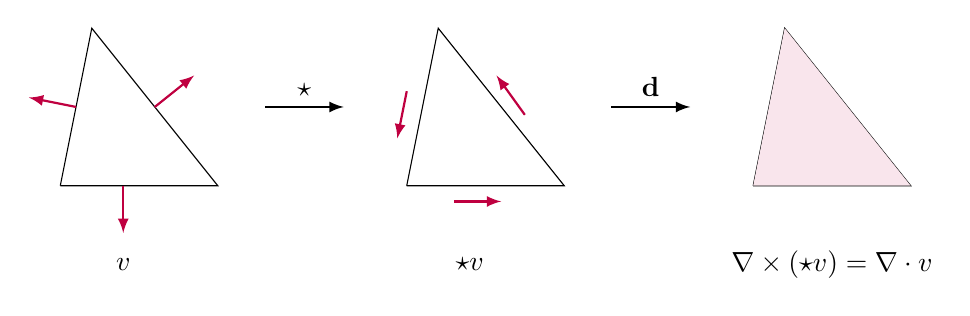
\begin{tikzpicture}[scale=2]
    \draw (0,0) -- (1,0) -- (0.2, 1) -- (0,0);
    \begin{scope}[thick,purple,->]
      \draw (0.4,-0.0) -- (0.4,-0.3);
      \draw (0.6,0.5) -- (0.85,0.7);
      \draw (0.1,0.5) -- (-0.2,0.56);
    \end{scope}
    \node at (0.4, -0.5) {$v$};
    \draw[thick,->] (1.3,0.5) -- node[above]{$\star$} (1.8,0.5);
    \begin{scope}[xshift=2.2cm]
      \draw (0,0) -- (1,0) -- (0.2, 1) -- (0,0);
      \begin{scope}[thick,purple,->]
        \draw (0.3,-0.1) -- (0.6,-0.1);
        \draw (0.75,0.45) -- (0.57,0.7);
        \draw (0.0,0.6) -- (-0.06,0.3);
      \end{scope}
      \node at (0.4,-0.5) {$\star v$};
      \draw[thick,->] (1.3,0.5) -- node[above]{$\mathbf{d}$} (1.8,0.5);
    \end{scope}
    \begin{scope}[xshift=4.4cm]
      \draw (0,0) -- (1,0) -- (0.2, 1) -- (0,0);
      \fill[purple!10] (0,0) -- (1,0) -- (0.2, 1) -- (0,0);
      \node at (0.5,-0.5) {$\nabla \times (\star v) = \nabla \cdot v$};
    \end{scope}
  \end{tikzpicture}
  \caption{2D divergence as the exterior derivative of a rotated form.}
  \label{fig:2d_divergence}
\end{figure}

Note that divergence expressed this way is a 2-form,
and we've chosen to represent $p$ as a 0-form.
To match the dimension of $p$, an additional Hodge star
needs to be applied to the divergence.
The first equation in \ref{eq:wave1stOrd} thus becomes
\begin{equation}\label{eq:intermediate_eq_1}
  \frac{\partial p}{\partial t} - c^2 \star \mathbf{d} \star v = 0.
\end{equation}

The second equation is more straightforward,
as the exterior derivative of a 0-form directly corresponds to the gradient.
In exterior calculs notation, it becomes
\begin{equation}\label{eq:intermediate_eq_2}
  \frac{\partial v}{\partial t} - \mathbf{d} p = 0.
\end{equation}

TODO: mention why the absorbing boundary condition is used

These equations are a good starting point, but we're not quite finished yet.
The problem arises from the absorbing boundary condition,
which will be covered in more detail in section \ref{sec:boundary_conditions}.
The boundary condition involves the \textit{flux} of velocity across the boundary,
meaning its component normal to the boundary, $\mathbf{v} \cdot \mathbf{n}$.
If we represent $v$ as a 1-cochain, integrating $v$ over boundary edges
in the tangent direction, information about the normal direction is lost.
Thus, to express this boundary condition,
we need to represent our equations in terms of flux instead of velocity.

In exterior calculus notation the flux is $\star v$.
The reason for this is the same as the reason
why divergence can be computed as the curl of $\star v$.
In a sense, the star turns a line integrated in the tangent direction
into a line integrated in the normal direction,
analogously to the 3D case where a 1-form (line)
turns into a 2-form (surface) integrated in the normal direction.

The final choices for the unknowns in our equations
are the 0-form pressure $p$
and the 1-form velocity flux $q = \star v$.
Substituting these variables into equations \eqref{eq:intermediate_eq_1}
and \eqref{eq:intermediate_eq_2} and applying one more Hodge star 
to \eqref{eq:intermediate_eq_2} yields the system
\begin{equation}
  \begin{cases}
    \frac{\partial p}{\partial t} - c^2 \star \mathbf{d} q = 0 \\
    \frac{\partial q}{\partial t} - \star \mathbf{d} p = 0 \\
  \end{cases}
\end{equation}


\section{Discretization}

Discretization of the model into a computer-solvable form
is performed separately for space and time.
The procedures defined by DEC are used for the spatial part,
and time discretization is performed using a staggered
finite difference scheme known as the leapfrog method.


\subsection{Space}

Spatial discretization in DEC is straightforward:
given a continuous model in exterior calculus notation,
a simplicial complex $\mathcal{K}$ approximating the domain $\Omega$ and its dual,
replace $k$-forms in the model with $k$-cochains,
$\mathbf{d}$ with the coboundary operator,
and $\star$ with the discrete Hodge star,
and you're most of the way done.
Denoting the 0-cochain equivalent of $p$ by $P$
and the 1-cochain equivalent of $q$ by $Q$,
this yields the semi-discrete equations
\begin{equation}\label{eq:semi_discrete_model}
  \begin{cases}
    \frac{\partial P}{\partial t} - c^2 \star \mathbf{d} Q = 0 \\
    \frac{\partial Q}{\partial t} - \star \mathbf{d} P = 0 \\
  \end{cases}
\end{equation}
(only \textit{semi}-discrete at this point
because they are still continuous in time).

The only remaining question is whether the cochains should be placed
on the primal mesh or the dual.
In our case, the implementation of boundary conditions demands $Q$
be available on the boundary edges, which means $Q$ must be on primal edges
(as dual edges are orthogonal to the boundary instead).
From there, $P$ should be placed such that the terms in equations \eqref{eq:semi_discrete_model}
are in the same cochain space.
In the first equation, $\star\mathbf{d}Q$
takes $Q$ from primal edges to primal faces and from there to dual vertices,
suggesting that $P$ should be a \textbf{dual} 0-cochain.
Checking that $\star \mathbf{d} P$ in the second equation
is a primal 1-cochain confirms this as the correct choice.

With these choices, we can pin down which forms of $\star$ and $\mathbf{d}$
are used in the system \eqref{eq:semi_discrete_model}.
Recall that given the matrices $\star_k$ and $\mathbf{d}_k$
defined in terms of the primal mesh,
the corresponding operators on the dual mesh are
$\star_k^{-1}$ and $\mathbf{d}_{n-k-1}$.
In terms of these operators, the system \eqref{eq:semi_discrete_model} becomes
\begin{equation}\label{eq:semi_discrete_model_annotated}
  \begin{cases}
    \frac{\partial P}{\partial t} - c^2 \star_1 \mathbf{d}_1 Q = 0 \\
    \frac{\partial Q}{\partial t} - \star_1^{-1} \mathbf{d}_1^T P = 0.
  \end{cases}
\end{equation}

To produce the cochain elements $P_i$ and $Q_i$
on the dual vertices $v_i^*$ and primal edges $\mathcal{E}_i$
from the continuous variables $p$ and $\mathbf{v}$,
we get the formulas
\begin{align}
  \label{eq:cochain_p}
  P_i &= p(v_i^*) \\
  \label{eq:cochain_q}
  Q_i &= \int_{\mathcal{E}_i} (\mathbf{v} \cdot \mathbf{n}) \,ds.
\end{align}
Note the term $\mathbf{v} \cdot \mathbf{n}$,
where $\mathbf{n}$ is the unit-length normal of the edge,
computing the flux of velocity in \eqref{eq:cochain_q}.


\subsection{Time}\label{sec:time_discr}

For time discretization we use the leapfrog method,
which is a second-order finite difference scheme
commonly used in ''Yee-like schemes''
(as termed by \textcite{rabina_numerical_2014}) such as DEC,
including \parencite{yee_numerical_1966} itself.
It is simple and efficient method,
requiring only one value of each variable to be computed per timestep.
See the lecture notes of \textcite{young_leapfrog_2014} for an explanation
of some of its desirable properties.

TODO: cite whoever first came up with ''Yee-like schemes''
instead of Räbinä (Bossavit, Kettunen)

In the leapfrog method, time advances in steps of $\Delta t$ seconds,
and values of $P$ and $Q$ are computed at separate time instances
offset from each other by $\frac{\Delta t}{2}$.
Let $t^k = k\Delta t$ denote the value of time after $k$ timesteps
and $P^k$ the value of $P$ at this time.
The next value of $Q$ is computed at the time $t^k + \frac{\Delta t}{2}$,
which we denote $Q^{k+\frac{1}{2}}$.
The time derivatives of $P$ and $Q$ are then approximated with
\begin{eqnarray}
  \label{eq:time_derivative_p}
  \frac{\partial P}{\partial t}(t^{k+\frac{1}{2}}) = \frac{P^{k+1} - P^k}{\Delta t} \\
  \label{eq:time_derivative_q}
  \frac{\partial Q}{\partial t}(t^k) = \frac{Q^{k+\frac{1}{2}} - Q^{k-\frac{1}{2}}}{\Delta t}
\end{eqnarray}

Substituting \eqref{eq:time_derivative_p} and \eqref{eq:time_derivative_q}
into \eqref{eq:semi_discrete_model_annotated} yields
\begin{align*}
\frac{P^{n+1} - P^n}{\Delta t} - c^2 \star_1 \mathbf{d}_1 Q^{n+\frac{1}{2}} &= 0 \\
\frac{Q^{n+\frac{3}{2}} - Q^{n+\frac{1}{2}}}{\Delta t}
- \star_1^{-1} \mathbf{d}_1^T P^{n+1} &= 0 \\
\end{align*}

Multiplying by $\Delta t$ and moving terms to the right-hand side
produces the timestep formulas
\begin{align}
  \label{eq:timestep_p}
  P^{n+1} &= P^n + \Delta t c^2 \star_1 \mathbf{d}_1 Q^{n+\frac{1}{2}} \\
  \label{eq:timestep_q}
  Q^{n+\frac{3}{2}} &= Q^{n+\frac{1}{2}} + \Delta t \star_1^{-1} \mathbf{d}_1^T P^{n+1}
\end{align}

This is an \textit{explicit} method:
the timestep formulas can be applied as matrix multiplications
to the values of $P$ and $Q$ at the beginning of a timestep,
without being required to solve any linear systems.
This makes the method computationally efficent and highly parallelizable,
but only conditionally stable.
There is an upper limit to the timestep $\Delta t$,
known as the \textit{Courant-Friedrichs-Lewy condition}
or CFL condition \parencite{courant_partial_1967},
above which the system will begin to gain energy and ''blow up'' towards infinity.
Determining the exact value of this condition is difficult
and we don't do it here, opting instead to find a stable value experimentally.

TODO: rephrase the last sentence


\section{Boundary conditions}\label{sec:boundary_conditions}

Our main test case models the scattering of acoustic waves
on impact with a so-called \textit{sound-soft} obstacle.
For this purpose we define two boundaries,
$\Gamma_{sca}$ for the scattering obstacle
and $\Gamma_{ext}$ for the outer boundary of the computational domain,
illustrated in figure \ref{fig:scatterer_domain}.

\begin{figure}[h]
  \centering
  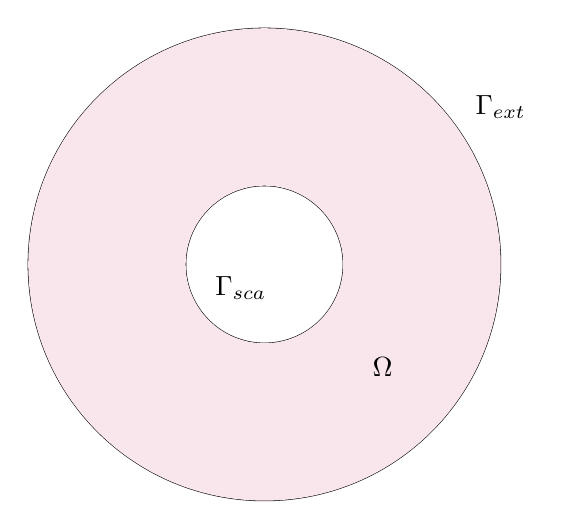
\begin{tikzpicture}
    \draw circle [radius=3];
    \draw circle [radius=1];
    \fill[fill=purple!10, even odd rule] circle [radius=3] circle [radius=1];
    \node at (3,2) {$\Gamma_{ext}$};
    \node at (-0.3,-0.3) {$\Gamma_{sca}$};
    \node at (1.5,-1.3) {$\Omega$};
  \end{tikzpicture}
  \caption{The domain $\Omega$ and boundaries $\Gamma_{ext}$ and $\Gamma_{sca}$
    of a scattering model.}
  \label{fig:scatterer_domain}
\end{figure}

Given an incident wave with velocity potential $\phi_{inc}$,
the scattering obstacle is modelled by setting $\phi_{inc}$ on $\Gamma_{sca}$
as a Dirichlet boundary condition
\begin{equation}
  \mathbf{v} = \nabla \phi_{inc}
  \quad \text{in } \Gamma_{sca} \times [0, T]
\end{equation}
where $[0,T]$ is the simulated time period.
The boundary condition is only applied to $\mathbf{v}$
and not $p$ because $p$ is placed on the dual mesh,
which does not have elements at the boundary.

On the outer boundary of the domain $\Gamma_{ext}$
we want the waves to travel out of the domain uninterrupted
in order to model the domain sitting inside a larger empty space.
This is accomplished using a first-order absorbing Engqvist-Majda boundary condition
\parencite{engquist_absorbing_1977}
\[
  \frac{1}{c}\frac{\partial\phi}{\partial t} + \mathbf{n} \cdot \nabla\phi = 0
  \quad \text{in } \Gamma_{ext} \times [0, T].
\]

Substituting the variables $p = \frac{\partial \phi}{\partial t}$
and $\mathbf{v} = \nabla \phi$ yields
\[
  \frac{1}{c}p + \mathbf{n} \cdot \mathbf{v} = 0,
\]
which translates to the differential form expression
\[
  \frac{1}{c}p + \star v = 0.
\]
Finally, we can substitute in our model variable $q = \star v$,
producing the boundary conditions
\begin{alignat}{2}
  \label{eq:boundary_dirichlet}
  q &= \star(\nabla \phi_{inc})^{\flat} & \qquad \text{in } \Gamma_{ext} \times [0, T] \\
  \label{eq:boundary_absorbing}
  \frac{1}{c} p + q &= 0 & \text{in } \Gamma_{sca} \times [0, T]
\end{alignat}

An issue with the absorbing boundary condition \eqref{eq:boundary_absorbing}
is that $p$ and $q$ exist on different mesh elements in our DEC model.
An approximation is needed to turn one of $p$ or $q$ into a form compatible with the other.
We use the same approximation used to define the discrete (Yee's) Hodge star,
the assumption of locally constant forms.

Specifically, we assume $p$ is constant over the primal face corresponding
to each dual vertex $P$ is stored on,
and therefore constant over the nearest boundary edge
when the primal face is adjacent to the boundary.
Denoting a boundary edge by $\mathcal{E}_i$,
the corresponding flux cochain element by $Q_i$
and the pressure of the adjacent face's dual vertex by $P_{\mathcal{E}_i}$,
the boundary condition \eqref{eq:boundary_absorbing} is approximated with
\[
  Q_i + \frac{1}{c} \int_{\mathcal{E}_i} P_{\mathcal{E}_i} ds = 0,
\]
leading to the flux update formula for boundary edges
\begin{equation}
  Q_i = -\frac{1}{c} |\mathcal{E}_i| P_{\mathcal{E}_i},
\end{equation}
where $|\mathcal{E}_i|$ is the length of the edge.


\section{Harmonic operators}\label{sec:harmonic_operators}

The time discretization of section \ref{sec:time_discr}
and the discrete Hodge star of section \ref{sec:discrete_hodge}
are based on linear and locally constant approximations.
However, in our case we know we're simulating harmonic waves,
which is a fact that can be used to derive more accurate approximations
of the time derivative and Hodge star.
The derivations in this section are adapted to our use case
from \parencite{rabina_numerical_2014}.

TODO: emphasize own contribution


\subsection{Exact time stepping}\label{sec:exact_timestep}

The state of a time-harmonic wave at timestep $k$ and time $t$
can be expressed in terms of complex exponentiation as
\begin{align}
\label{eq:harmonic_pressure}
P(t) &= \text{Re}(\hat{P}_0 \exp(-i\omega t)) \\
\label{eq:harmonic_flux}
Q(t + \frac{\Delta t}{2}) &= \text{Re}(\hat{Q}_0 \exp(-i\omega (t + \frac{\Delta t}{2}))
\end{align}
where $\hat{P}_0$ and $\hat{Q}_0$ are complex initial values for $P$ and $Q$,
$\omega$ is the angular velocity of the wave, and $i$ is the imaginary unit.

Substituting \eqref{eq:harmonic_pressure}
into the numerator of equation \eqref{eq:time_derivative_p}
where $t^k = t + \frac{\Delta t}{2}$, we get
\begin{align*}
& P(t^k + \frac{\Delta t}{2}) - P(t^k - \frac{\Delta t}{2}) \\
&= \text{Re} \Big[ \hat{P}_0 \exp(-i\omega (t^k + \frac{\Delta t}{2})) \Big]
- \text{Re} \Big[ \hat{P}_0 \exp(-i\omega (t^k - \frac{\Delta t}{2}) \Big] \\
&= \text{Re} \Big[ \hat{P}_0 (\exp(-i\omega (t^k + \frac{\Delta t}{2}))
- \exp(-i\omega (t^k - \frac{\Delta t}{2})) \Big] \\
&= \text{Re} \Big[ \hat{P}_0 \exp(-i\omega t^k)
\Big( \exp(-i\omega \frac{\Delta t}{2}) - \exp(i\omega \frac{\Delta t}{2}) \Big) \Big] \\
&= \text{Re} \Big[ -i\omega \hat{P}_0 \exp(-i\omega t^k)
\Big(\frac{\exp(-i\omega \frac{\Delta t}{2}) - \exp(i\omega \frac{\Delta t}{2})}{-i\omega}\Big) \Big] \\
&= \text{Re} \Big[ \frac{\partial P}{\partial t}(t^k)
\Big(\frac{\exp(-i\omega \frac{\Delta t}{2}) - \exp(i\omega \frac{\Delta t}{2})}{-i\omega}\Big) \Big] \\
&= - \frac{1}{\omega} \frac{\partial P}{\partial t}(t^k)
\cdot \text{Im} \Big[\exp(-i\omega \frac{\Delta t}{2}) - \exp(i\omega \frac{\Delta t}{2}) \Big] \\
&= \frac{\partial P}{\partial t}(t^k) \Big(\frac{2}{\omega} \sin(\frac{\omega \Delta t}{2}) \Big).
\end{align*}

TODO: see if some intermediate steps should be omitted

The same consideration for the flux \eqref{eq:harmonic_flux}
produces the same coefficient.

With this, the time derivative approximations \eqref{eq:time_derivative_p}
and \eqref{eq:time_derivative_q} become
\begin{align}
\label{eq:time_derivative_p_har}
\frac{\partial P}{\partial t}
&= \frac{P^{n+1} - P^n}{\frac{2}{\omega}\sin\frac{\omega \Delta t}{2}} \\
\label{eq:time_derivative_q_har}
\frac{\partial Q}{\partial t}
&= \frac{Q^{n+\frac{3}{2}} - Q^{n+\frac{1}{2}}}{\frac{2}{\omega}\sin\frac{\omega \Delta t}{2}}
\end{align}
and the timestep equations \eqref{eq:timestep_p} and \eqref{eq:timestep_q}
\begin{align}
\label{eq:timestep_p_har}
P^{n+1} &= P^n
+ \frac{2}{\omega}\sin\frac{\omega \Delta t}{2} (c^2 \star_2 d_1 Q^{n+\frac{1}{2}}) \\
\label{eq:timestep_q_har}
Q^{n+\frac{3}{2}} &= Q^{n+\frac{1}{2}}
+ \frac{2}{\omega}\sin\frac{\omega \Delta t}{2} (\star_1^{-1} d_1^T P^{n+1}).
\end{align}

TODO: original source for this


\subsection{Harmonic Hodge star}\label{sec:harmonic_hodge}

The harmonic properties of acoustic waves also apply to space.
In a small neighborhood around any given point,
it can be assumed that the solution behaves like a complex plane wave
\begin{equation}\label{eq:plane_wave}
  \hat{u}(\mathbf{x}) = \hat{u}_0 \exp(i\vec{\kappa} \cdot \mathbf{x})
\end{equation}
where $\hat{u}_0$ is a complex initial value,
and $\vec{\kappa}$ is the \textit{wave vector} $\kappa \mathbf{d}$,
where in turn $\mathbf{d}$ is the unit-length direction of wave propagation
and $\kappa$ is the \textit{wavenumber}.
The wavenumber is the number of wave periods per unit of distance,
related to the wavelength $\lambda$ by $\kappa = \frac{2\pi}{\lambda}$
and the angular velocity $\omega$ and propagation speed $c$ by
$\kappa = \frac{\omega}{c}$.

\textbf{Edge to edge}

In the case of $\star_1$ taking a 1-cochain from a flux on the primal edge $\mathcal{E}$
to a veloctity on the dual edge $\mathcal{E}^*$,
we would like to minimize the error
\begin{equation}\label{eq:harmonic_error_norm}
  ||\int_{\mathcal{E}} \hat{u} \cdot \mathbf{n} \,ds
  - \star_1^{-1} \int_{\mathcal{E}^*} \hat{u} \cdot \mathbf{t} \,ds\,||^2
\end{equation}
where $\mathbf{n}$ is the unit normal vector to $\mathcal{E}$
and $\mathbf{t}$ is the unit tangent vector to $\mathcal{E}^*$.
Denoting $\hat{u}_{\mathcal{E}} = \int_{\mathcal{E}} \hat{u} \cdot \mathbf{n} \,ds$
and $\hat{u}_{\mathcal{E}^*} = \int_{\mathcal{E}^*} \hat{u} \cdot \mathbf{t} \,ds$,
this gives the quadratic equation
\[
\hat{u}_{\mathcal{E}}^2
- 2 \star_1^{-1} \hat{u}_{\mathcal{E}} \hat{u}_{\mathcal{E}^*}
+ (\star_1^{-1})^2 \hat{u}_{\mathcal{E}^*}^2,
\]
the derivative of which with respect to $\star_1$ is
\[
  2 \star_1^{-1} \hat{u}_{\mathcal{E}^*}^2 - 2 \hat{u}_{\mathcal{E}} \hat{u}_{\mathcal{E}^*},
\]
which is zero and thus the error is minimized when
\[
  \star_1^{-1} = \frac{\hat{u}_{\mathcal{E}} \hat{u}_{\mathcal{E}^*}}{\hat{u}_{\mathcal{E}^*}^2}
  \iff \star_1 = \frac{\hat{u}_{\mathcal{E}^*}^2}{\hat{u}_{\mathcal{E}} \hat{u}_{\mathcal{E}^*}}.
\]

However, this only applies when the propagating direction $\mathbf{d}$
is a known constant, which is generally not true.
For practical cases, we need to minimize this error
over all possible propagating directions.
This is accomplished by integrating $\mathbf{d}$ over the unit circle
in polar coordinates, where $\mathbf{d} = (\cos\theta, \sin\theta)$,
resulting in the formula
\begin{equation}\label{eq:star_1_integral}
  \star_1 = \frac{\int_{0}^{2\pi} \hat{u}_{\mathcal{E}^*}^2 \,d\theta}
  {\int_{0}^{2\pi} \hat{u}_{\mathcal{E}} \hat{u}_{\mathcal{E}^*} \,d\theta}.
\end{equation}

For the following computation, we assume $\mathcal{E}$ and $\mathcal{E}^*$
are orthogonal and centered at the origin.
Due to the symmetry of the unit circle, orientation of the edges has no effect
and thus we can also assume $\mathcal{E}$ is oriented along the x-axis
and $\mathcal{E}^*$ along the y-axis.
Using the Taylor series $\exp(ax) = \sum_{n=0}^{\infty} \frac{a^nx^n}{n!}$
and the auxiliary variable $\alpha = i\kappa\cos\theta$, we get
\begin{align*}
\hat{u}_{\mathcal{E}} &= \int_{\mathcal{E}} \hat{u} \cdot \mathbf{n} \,ds \\
&= (\hat{u}_0)_y \int_{-\frac{l}{2}}^{\frac{l}{2}} \exp(i \kappa x \cos\theta) \,dx \\
&= (\hat{u}_0)_y \int_{-\frac{l}{2}}^{\frac{l}{2}} \sum_{n=0}^{\infty} \frac{\alpha^n x^n}{n!} \,dx \\
&= (\hat{u}_0)_y \Big[ \sum_{n=0}^{\infty} \frac{1}{n}\frac{\alpha^n x^{n+1}}{n!} \Big]_{x = -\frac{l}{2}}^{x = \frac{l}{2}} \\
&= (\hat{u}_0)_y \sum_{n=0}^{\infty} \frac{\alpha^n \Big( (\frac{l}{2})^{n+1} - (-\frac{l}{2})^{n+1} \Big)}{(n + 1)!} \\
&\text{(terms where $n$ is odd are eliminated)} \\
&= (\hat{u}_0)_y \sum_{n=0}^{\infty} \frac{\alpha^{2n} 2(\frac{l}{2})^{2n+1}}{(2n + 1)!} \\
&= (\hat{u}_0)_y \sum_{n=0}^{\infty} \frac{\alpha^{2n} l^{2n+1}}{2^{2n}(2n + 1)!} \\
&= (\hat{u}_0)_y l \sum_{n=0}^{\infty} \frac{(\alpha l)^{2n}}{2^{2n}(2n + 1)!}
\end{align*}
where $l$ is the length of $\mathcal{E}$
and $(\hat{u}_0)_y$ is the y component of $\hat{u}_0$.

Similarly, the exponential term for $\hat{u}_{\mathcal{E}^*}$
and the same integration produces
\[
  \hat{u}_{\mathcal{E}^*} = (\hat{u}_0)_y l^* \sum_{n=0}^{\infty} \frac{(\beta l^*)^{2n}}{2^{2n}(2n + 1)!}. 
\]
where $l^*$ is the length of $\mathcal{E}^*$.

The first few terms of this series are
\[
  \hat{u}_{\mathcal{E}} = (\hat{u}_0)_y l
  \Big( 1 + \frac{(\alpha l)^2}{24} + \frac{(\alpha l)^4}{1920} + \dots \Big)
\]
and the y component of $\hat{u}_0$ is $(u_0)_y = u_0\sin\theta$,
where $u_0 = |\hat{u}_0|$ is the magnitude of $\hat{u}_0$.

With these series expressions we can build the products
in the optimized Hodge star as series
whose first few terms are
\begin{align*}
\hat{u}_{\mathcal{E}^*}^2 &= u_0^2 (\sin^2\theta) (l^*)^2
\Big( 1 + \frac{(\beta l^*)^2}{12} + \frac{(\beta l^*)^4}{360} + \dots \Big) \\
\hat{u}_{\mathcal{E}} \hat{u}_{\mathcal{E}^*} &= u_0^2 (\sin^2\theta) ll^*
\Big( 1 + \frac{(\alpha l)^2}{24} + \frac{(\beta l^*)^2}{24}
+ \frac{(\alpha l \beta l^*)^2}{576} + \dots \Big).
\end{align*}

Now we need to integrate these expressions around the unit circle.
First, we can get rid of the imaginary terms in $\alpha$ and $\beta$
by evaluating the even powers.
Switching notation to denote the edge lengths
by $|\mathcal{E}|$ and $|\mathcal{E}^*|$, we get
\begin{align*}
  (\alpha l)^2 &= -\kappa^2 |\mathcal{E}|^2 \cos^2 \theta \\
  (\beta l^*)^2 &= -\kappa^2 |\mathcal{E}^*|^2 \sin^2 \theta.
\end{align*}

Substituting these values we get the integrals
\begin{align*}
\int_{0}^{2\pi} \hat{u}_{\mathcal{E}^*}^2 \,d\theta
&= u_0^2 |\mathcal{E}^*|^2 \int_{0}^{2\pi}
\Big( sin^2\theta - \frac{\kappa^2 |\mathcal{E}^*|^2 \sin^4\theta}{12}
+ \frac{\kappa^4 |\mathcal{E}^*|^4 \sin^6\theta}{360} + \dots \Big) \,d\theta \\
&= u_0^2 |\mathcal{E}^*|^2 \pi \Big(
1 - \frac{\kappa^2 |\mathcal{E}^*|^2}{16}) \Big)
+ \mathcal{O}(\kappa^4 |\mathcal{E}^*|^4)\\
\\
\int_{0}^{2\pi} \hat{u}_{\mathcal{E}} \hat{u}_{\mathcal{E}^*} \,d\theta
&= u_0^2 |\mathcal{E}| |\mathcal{E}^*| \int_{0}^{2\pi}
\Big( \sin^2\theta - \frac{\kappa^2 |\mathcal{E}|^2 \sin^2\cos^2\theta}{24}
- \frac{\kappa^2 |\mathcal{E}^*|^2 \sin^4\theta}{24} \\
&\qquad\qquad\qquad\qquad + \frac{\kappa^4 |\mathcal{E}|^2 |\mathcal{E}^*|^2
  \sin^4\cos^2\theta}{576} + \dots \Big) \,d\theta \\
&= u_0^2 |\mathcal{E}| |\mathcal{E}^*| \pi \Big(
1 - \frac{\kappa^2 |\mathcal{E}|^2}{96} - \frac{\kappa^2 |\mathcal{E}^*|^2}{32} \Big)
+ \mathcal{O}(\kappa^4 |\mathcal{E}|^2 |\mathcal{E}^*|^2)
\end{align*}

Dividing these according to equation \eqref{eq:star_1_integral} yields
\begin{equation}\label{eq:harmonic_hodge_1}
  \star_1 \approx \frac{|\mathcal{E}^*|}{|\mathcal{E}|}
  \Big( \frac{1 - \frac{\kappa^2 |\mathcal{E}^*|^2}{16}}
  { 1 - \frac{\kappa^2 |\mathcal{E}|^2}{96} - \frac{\kappa^2 |\mathcal{E}^*|^2}{32} } \Big).
\end{equation}

\textbf{Face to vertex}

The same consideration for $\star_2$ taking a 2-cochain
on a primal face $\mathcal{F}$ to a 0-cochain 
on a dual vertex $v^*$ yields
\begin{equation}\label{eq:star_2_integral}
  \star_2 = \frac{\int_0^{2\pi} \hat{u}(v^*)^2 \,d\theta}
  {\int_0^{2\pi} \hat{u}_{\mathcal{F}} \hat{u}(v^*) \,d\theta}
\end{equation}

where $\hat{u}_{\mathcal{F}}$ is the wave \eqref{eq:plane_wave}
integrated over the face and $\hat{u}(v^*)$ is the wave evaluated at the vertex.
We can assume for now that the vertex is at the origin
and the face is a circle with radius $r$ and area $\pi r^2$.
A generalization for polygon faces will be performed later.

The vertex being at the origin implies $\hat{u}(v^*) = \hat{u}(0) = \exp(0) = 1$.

The integral of $\hat{u}$ over the circular face $\mathcal{F}$ is
symmetric for all angles $\theta$, so we may assume $\theta = \frac{\pi}{2}$,
i.e. that the wave is propagating along the y-axis.
We then have
\begin{align*}
  \hat{u}_{\mathcal{F}} &= \int_{\mathcal{F}} \hat{u} \\
  &= \int_{-r}^{r} \int_{-\sqrt{r^2 - x^2}}^{\sqrt{r^2 - x^2}}
    \exp(i\kappa y) \,dydx \\
  &= \int_{-r}^{r} \int_{-\sqrt{r^2 - x^2}}^{\sqrt{r^2 - x^2}}
    \sum_{n=0}^{\infty} \frac{(i\kappa)^n y^n}{n!} \,dydx \\
  &= \int_{-r}^{r} \sum_{n=0}^{\infty}
    \frac{(i\kappa)^n \Big((\sqrt{r^2 - x^2})^{n+1} - (-\sqrt{r^2 - x^2})^{n+1} \Big)}{(n + 1)!} \,dx \\
  &\text{(terms where $n$ is odd are eliminated)} \\
  &= \int_{-r}^{r} \sum_{n=0}^{\infty} \frac{2 (i\kappa)^{2n} (\sqrt{r^2 - x^2})^{2n+1}}{(2n + 1)!} \,dx.
\end{align*}

Here we change the variable to $t$ such that $x = r\sin t$,
for which $dx = r\cos t dt$ and $\sqrt{r^2 - x^2} = r\cos t$,
and continue to integrate the first few terms of the series:
\begin{align*}
\hat{u}_{\mathcal{F}}
&= \int_{-\frac{\pi}{2}}^{\frac{\pi}{2}}
  \sum_{n=0}^{\infty} \frac{2(i\kappa)^{2n} (r\cos t)^{2n+1}}{(2n + 1)!} r\cos t \,dt \\
&= \sum_{n=0}^{\infty} \frac{2(i\kappa)^{2n} r^{2n+2}}{(2n + 1)!}
  \int_{-\frac{\pi}{2}}^{\frac{\pi}{2}} (\cos t)^{2n+2} \,dt \\
&= \pi r^2 \Big( 1 + \frac{(i\kappa r)^2}{8} + \frac{(i\kappa r)^4}{192} + \dots \Big)
\end{align*}

Integrating $\hat{u}_{\mathcal{F}} \hat{u}(v^*)$ over the unit circle,
evaluating the $i^2$ terms,
and substituting $|\mathcal{F}| = \pi r^2$ gives
\begin{align*}
\int_{0}^{2\pi} \hat{u}_{\mathcal{F}} \hat{u}(v^*) \,d\theta
&\approx |\mathcal{F}| \int_{0}^{2\pi}
  \Big( 1 - \frac{(\kappa r)^2}{8} + \frac{(\kappa r)^4}{192} + \dots \Big) \,d\theta \\
&= 2\pi |\mathcal{F}| \Big( 1 - \frac{(\kappa r)^2}{8} \Big)
+ \mathcal{O}(\frac{(\kappa r)^4}{192}).
\end{align*}

Because $\hat{u}(v^*)^2$ is the constant 1, its integral over the unit circle is $2\pi$.
It then follows from equation \eqref{eq:star_2_integral} that
\begin{equation}\label{eq:star_2_harmonic}
  \star_2 \approx \frac{1}{|\mathcal{F}|}
  \Big( \frac{1}{1 - \frac{(\kappa r)^2}{8}} \Big).
\end{equation}

\textbf{Polygon faces}

The preceding derivation was based on circular faces,
but the faces in practical applications are polygons.
We can make use of results obtained from the circle case
by approximating polygons with circles.

Given a regular polygon with maximum internal sphere radius $r$
and minimum external sphere radius $R$,
performing the integrations of equation \eqref{eq:star_2_integral}
over a triangle or square
using the approximation $r^2_{\mathcal{F}} = \frac{1}{3} (2r^2 + R^2)$
matches the first three terms of the Taylor polynomial obtained from the circle case.

With irregular convex polygons, each edge defines a different value for $r$
and each vertex a different value for $R$,
as illustrated in figure \ref{fig:polygon_radii}.
$r_k$ is the perpendicular distance from the origin to the edge $k$
and $R_k$ is the distance to the vertex $k$.

\begin{figure}[h]
  \centering
  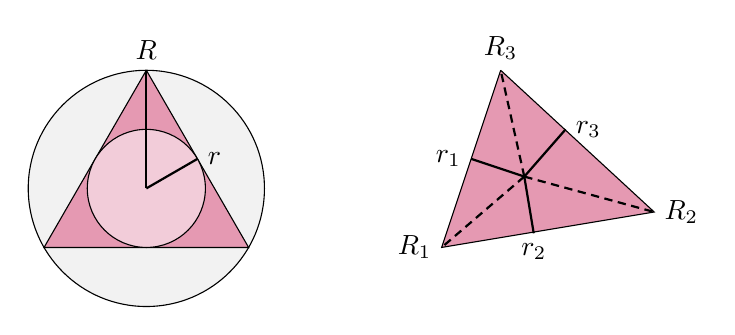
\begin{tikzpicture}[scale=1.5]
    \draw[fill=black!5] circle[radius=1];
    \draw[fill=purple!40] (0,1) -- ({cos(210)},{sin(210)}) -- ({cos(-30)},{sin(-30)}) -- (0,1);
    \draw[fill=purple!20] circle[radius=0.5];
    \draw[thick] (0,0) -- (0,1) node[above]{$R$};
    \draw[thick] (0,0) -- ({0.5*cos(30)},{0.5*sin(30)}) node[right]{$r$};
    \begin{scope}[xshift=3cm]
      \draw[fill=purple!40] (0,1) -- (-0.5, -0.5) -- (1.3,-0.2) -- (0,1);
      \begin{scope}[thick]
        \draw (0.2,0.1) -- (-0.25,0.25) node[left]{$r_1$};
        \draw[densely dashed] (0.2,0.1) -- (-0.5,-0.5) node[left]{$R_1$};
        \draw (0.2,0.1) -- (0.28,-0.38) node[below]{$r_2$};
        \draw[densely dashed] (0.2,0.1) -- (1.3, -0.2) node[right]{$R_2$};
        \draw (0.2,0.1) -- (0.55,0.5) node[right]{$r_3$};
        \draw[densely dashed] (0.2,0.1) -- (0,1) node[above]{$R_3$};
      \end{scope}
    \end{scope}
  \end{tikzpicture}
  \caption{Internal and external radii of a regular and irregular triangle.}
  \label{fig:polygon_radii}
\end{figure}

The approximation we use for irregular polygons with $n$ edges is the average
of the regular polygon approximations corresponding to each edge
\begin{equation}\label{eq:polygon_approx_radius}
  r^2_{\mathcal{F}} \approx \frac{1}{3n} \sum_{k=1}^n (2r_k^2 + R_k^2).
\end{equation}
Substituting this expression for $r^2$ in equation \eqref{eq:star_2_harmonic}
produces the $\star_2$ operator we use in our experiments.


\chapter{Exact controllability}\label{cha:controllability}

We use a solver based on discrete exterior calculus to simulate
a wave system forward in time.
In addition to this, we're interested in finding a state that is
\textit{time-periodic} in the entire domain $\Omega$,
meaning that the state of the simulation repeats at intervals of $T$ seconds.
Under the right circumstances, this can be achieved with our time-dependent solver
by simply running it for a long enough time period.
This is called the \textit{asymptotic iteration method}
because the time-periodic state is approached over time as $t \rightarrow \infty$.

A solution becomes time-periodic when all waves produced by a source
have reached an absorbing material or boundary.
This can only happen if all wave sources are time-periodic with period $T$
and all waves propagating from the sources are able to be absorbed by something.
Even when these conditions are fulfilled,
convergence of the asymptotic iteration can be slow or unreliable in cases
where waves spend a long time reflecting off surfaces before being absorbed,
as we find in the experiments of chapter \ref{cha:experiments}.

To accelerate convergence towards a time-periodic state,
we employ the concept of exact controllability
developed by \textcite{lions_exact_1988}
and first applied to the computation of time-periodic solutions by
\textcite{bristeau_controllability_1998}.
Our controllability method formulates the difference between 
the initial state at $t=0$ and the state at $t=T$
as a least-squares optimization problem
with the initial state as the variable to be optimized,
which is solved using the \textit{conjugate gradient} (CG) algorithm.
The gradients needed for this algorithm are obtained
using the \textit{adjoint state} method.


\section{Optimization problem}

Let $U^n = (P^n, Q^{n+1})^T$ be the state of the simulation at timestep $n$,
$\mathbf{e} = U^0$ the initial state, and $N$ the number of timesteps
required to simulate the time period $T$.
We want to find a state where $U^N - \mathbf{e} = 0$,
which is equivalent to minimizing the quadratic function
\begin{equation}\label{eq:control_energy}
  J(\mathbf{e}) = \frac{1}{2}(U^N - \mathbf{e})^T (U^N - \mathbf{e}).
\end{equation}

We call $J(\mathbf{e})$ the \textit{control energy}.
To solve this problem, we first need the gradient of $J$.


\section{Computing the gradient}

To compute the gradient $\nabla J(\mathbf{e})$,
we first need an expression for $U^N$.
This is accomplished by expressing the timestepping procedure
as a matrix multiplication and repeatedly applying it
until the end of the time window $T$.
This expression is used to expand the product in equation \eqref{eq:control_energy}
into a standard quadratic equation and find its gradient by inspection.


\subsection{State equation}

Inside of the domain $\Omega$, a single timestep
using the formulas \eqref{eq:timestep_p} and \eqref{eq:timestep_q}
can be expressed as the block matrix equation
\[
  \begin{bmatrix}
  I & \Delta t c^2 \star_2 d_1 & -I \\
  & I & \Delta t \star_1^{-1} d_1^T & -I
  \end{bmatrix}
  \begin{bmatrix}
  P^n \\ Q^{n+\frac{1}{2}} \\ P^{n+1} \\ Q^{n+\frac{3}{2}}
  \end{bmatrix}
  = 0.
\]

This can be extended to the entire time window $[0,T]$
by applying it repeatedly for $N$ timesteps, producing the equation
\begin{equation}\label{eq:state_equation}
  S(\mathbf{e}) =
  \begin{bmatrix}
  I \\
  \mathcal{C} & \mathcal{D} \\
  & \mathcal{C} & \mathcal{D} \\
  & & \ddots & \ddots \\
  & & & \mathcal{C} & \mathcal{D} \\
  & & & & \mathcal{C} & \mathcal{D} \\
  \end{bmatrix}
  \begin{bmatrix}
  U^0 \\ U^1 \\ \vdots \\ U^{N-1} \\ U^N
  \end{bmatrix}
  - \begin{bmatrix}
  \mathbf{e} \\ 0 \\ \vdots \\ 0 \\ 0
  \end{bmatrix}
  + \begin{bmatrix}
  0 \\ \mathcal{F}^0 \\ \vdots \\ \mathcal{F}^{N-2} \\ \mathcal{F}^{N-1}
  \end{bmatrix}
  = 0
\end{equation}
where
\[
  \mathcal{C} = \begin{bmatrix}
  I & \Delta t c^2 \star_2 d_1 \\
  0 & I
  \end{bmatrix},
  \quad
  \mathcal{D} = \begin{bmatrix}
  -I & 0 \\
  \Delta t \star_1^{-1} d_1^T & -I
  \end{bmatrix},
\]
and the vectors $\mathcal{F}^n$ contain source terms,
which in our case only include the values of the Dirichlet boundary condition
\eqref{eq:boundary_dirichlet} on the boundary $\Gamma_{sca}$.
Equation \eqref{eq:state_equation} is called the \textit{state equation}.

The domain boundaries need some special attention here,
as the equation as stated above does not apply to them.
The details are left out of \eqref{eq:state_equation} for clarity,
but it should be understood that rows of this equation
corresponding to mesh edges on the scattering obstacle's boundary $\Gamma_{sca}$
are replaced with rows that only have $(-1)$ on the diagonal.
Similarly, rows corresponding to edges on the absorbing boundary $\Gamma_{ext}$
are replaced with the matrix form of equation \eqref{eq:boundary_absorbing}.

Denoting $Q = -\mathcal{D}^{-1} \mathcal{C}$,
a single timestep in this matrix notation consists of the formula
\begin{equation}\label{eq:forward_timestep_matrix}
  U^{k+1} = -\mathcal{D}^{-1} (\mathcal{C} U^k + \mathcal{F}^k).
\end{equation}
Applying this $N$ times to the initial conditions $\mathbf{e}$ 
gives the expression for $U^N$
\begin{equation}\label{eq:final_state_matrix}
  U^N = Q^N \mathbf{e}
  - \sum_{i=0}^{N-1} Q^i \mathcal{D}^{-1} \mathcal{F}^{(N-1)-i}
\end{equation}
where $Q^n$ denotes the $n$th power of the square matrix $Q$.

\subsection{Gradient of control energy}

Equation \eqref{eq:final_state_matrix} allows us to formulate
a matrix expression for the gradient $\nabla J(\mathbf{e})$.
Let $\mathbf{g} = \sum_{i=0}^{N-1} Q^i \mathcal{D}^{-1} \mathcal{F}^{(N-1)-i}$,
which is a vector of the same dimension as $\mathbf{e}$.
An expanded form of the control energy is then
\begin{align*}
  J(\mathbf{e})
  &= \frac{1}{2} (U^N - \mathbf{e})^T (U^N - \mathbf{e}) \\
  &= \frac{1}{2} ((Q^N - I) \mathbf{e} - \mathbf{g})^T ((Q^N - I) \mathbf{e} - \mathbf{g}) \\
  &= \frac{1}{2} \mathbf{e}^T (Q^N - I)^T (Q^N - I) \mathbf{e} \\
  &\qquad -\, \frac{1}{2} (\mathbf{e}^T (Q^N - I)^T \mathbf{g}
    - \mathbf{g}^T (Q^N - I)\mathbf{e}) \\
  &\qquad +\, \frac{1}{2} \mathbf{g}^T \mathbf{g} \\
  &= \frac{1}{2} \mathbf{e}^T (Q^N - I)^T (Q^N - I) \mathbf{e}
  - \mathbf{g}^T (Q^N - I)\mathbf{e}
  + \frac{1}{2} \mathbf{g}^T \mathbf{g} \\
  &=: \frac{1}{2}\mathbf{e}^T A \mathbf{e} - \mathbf{b}^T \mathbf{e} + c,
\end{align*}
which gives us the gradient
\begin{equation}\label{eq:control_gradient}
  \nabla J(\mathbf{e}) = A\mathbf{e} - \mathbf{b}
\end{equation}
where
\[
  A = (Q^N - I)^T (Q^N - I),
  \quad b = \mathbf{g}^T (Q^N - I).
\]


\subsection{Adjoint state method}\label{sec:adjoint_state_method}

The obvious way to compute $\nabla J(\mathbf{e})$ would be either by
explicitly computing the matrix $A$ in equation \eqref{eq:control_gradient}
or by approximating it with finite differences.
However, these are both highly expensive procedures,
requiring $N$ large matrix multiplications in the first case
and $\dim(\mathbf{e})$ simulations up to time $T$ in the second.
The adjoint state method provides an efficient alternative,
requiring only one forward simulation to time $T$
and one \textit{backward} simulation back from time $T$ to time zero.
It states that
\begin{equation}\label{eq:adjoint_state_gradient}
  \frac{dJ}{d\mathbf{e}}
  = \frac{\partial J}{\partial \mathbf{e}}
  - \mathbf{z}^T \frac{\partial S}{\partial \mathbf{e}}
\end{equation}
where $S$ is the state equation \eqref{eq:state_equation}
and $\mathbf{z}$ is the solution to the \textit{adjoint equation}
\begin{equation}\label{eq:adjoint_equation}
  \Big(\frac{\partial S}{\partial \mathbf{u}}\Big)^T \mathbf{z}
  = \Big(\frac{\partial J}{\partial \mathbf{u}}\Big)^T.
\end{equation}
$\mathbf{z} = (Z^0, \dots, Z^N)^T$ is called the \textit{adjoint state variable}
and has the same dimension as the state variable
$\mathbf{u} = (U^0, \dots, U^N)^T$ in the state equation.

See \parencite{bradley_pde-constrained_2019} for a brief tutorial on the topic
and proof of the preceding statements, or \parencite{givoli_tutorial_2021}
for a more comprehensive introduction.

Because $U^n$ is the only state variable that exists in the control energy $J$,
\[
  \Big(\frac{\partial J}{\partial \mathbf{u}}\Big)^T = \begin{bmatrix}
    0 \\ 0 \\ \vdots \\ 0 \\ \Lambda(U^N - \mathbf{e})
  \end{bmatrix}.
\]

Similarly, because $\mathbf{e}$ is only present in the first row
of the state equation,
\[
  \frac{\partial S}{\partial \mathbf{e}} = (-I, 0, 0, \dots, 0)^T
\]
and thus 
\[
  \mathbf{z}^T \frac{\partial S}{\partial \mathbf{e}} = -Z^0.
\]
We also know that
\[
  \frac{\partial J}{\partial \mathbf{e}} = -(U^N - \mathbf{e}).
\]
It follows from substituting these values into equation \eqref{eq:adjoint_state_gradient}
that the gradient we're looking for is
\begin{equation}\label{eq:adjoint_solution}
  \frac{dJ}{d\mathbf{e}} = -(U^N - \mathbf{e}) + Z^0.
\end{equation}

To compute this we need the value of $Z^0$,
which can be obtained using the adjoint equation \eqref{eq:adjoint_equation}.
The matrix form of this equation looks very similar to the state equation:
\begin{equation}\label{eq:adjoint_equation_matrix}
  \begin{bmatrix}
    I & \mathcal{C}^T \\
    & \mathcal{D}^T & \mathcal{C}^T \\
    & & \mathcal{D}^T & \mathcal{C}^T \\
    & & & \ddots & \ddots \\
    & & & & \mathcal{D}^T & \mathcal{C}^T \\
    & & & & & \mathcal{D}^T \\
  \end{bmatrix}
  \begin{bmatrix}
    Z^0 \\ Z^1 \\ \vdots \\ Z^{N-1} \\ Z^N
  \end{bmatrix}
  = \begin{bmatrix}
    0 \\ 0 \\ \vdots \\ 0 \\ U^N - \mathbf{e}
  \end{bmatrix}
\end{equation}
where $\mathcal{C}$ and $\mathcal{D}$ are the block matrices
from the state equation \eqref{eq:state_equation}.

This equation can be solved with a backward procedure starting with
\begin{equation}\label{eq:adjoint_sim_start}
  Z^N = (\mathcal{D}^T)^{-1} (U^N - \mathbf{e}),
\end{equation}
followed by repeating
\begin{equation}\label{eq:adjoint_sim_step}
  Z^k = -(\mathcal{D}^T)^{-1} \mathcal{C}^T Z^{k+1}
\end{equation}
for $k = N-1, \dots, 1$ and finally
\begin{equation}\label{eq:adjoint_sim_final}
  Z^0 = -\mathcal{C}^T Z^1.
\end{equation}

Written out explicitly, a single timestep
according to equation \eqref{eq:adjoint_sim_step} looks like
\begin{align*}
  Z^k &= -(\mathcal{D}^T)^{-1} \mathcal{C}^T Z^{k+1} \\
  &= -\begin{bmatrix}
    -I & (\Delta t \star_1^{-1} d_1^T)^T \\
    0 & -I \\
  \end{bmatrix}^{-1}
  \begin{bmatrix}
    I & 0 \\
    (\Delta t c^2 \star_2 d_1)^T & I \\
  \end{bmatrix}
  \begin{bmatrix}
    z_0^{k+1} \\ z_1^{k+1}
  \end{bmatrix},
\end{align*}
which is equivalent to solving the equation
\[
  \begin{bmatrix}
    -I & (\Delta t \star_1^{-1} d_1^T)^T \\
    0 & -I \\
  \end{bmatrix}
  \begin{bmatrix}
    z_0^k \\ z_1^k
  \end{bmatrix}
  = -\begin{bmatrix}
    I & 0 \\
    (\Delta t c^2 \star_2 d_1)^T & I \\
  \end{bmatrix}
  \begin{bmatrix}
    z_0^{k+1} \\ z_1^{k+1}
  \end{bmatrix},
\]
producing the backward timestep formulas
\begin{align}
z_1^k &= z_1^{k+1} + (\Delta t c^2 \star_2 d_1)^T z_0^{k+1} \\
z_0^k &= z_0^{k+1} + (\Delta t \star_1^{-1} d_1^T)^T z_1^k.
\end{align}

Because the state equation is solved forward in time
and the adjoint state equation backward,
these equations are often called
the \textit{forward problem} and \textit{backward problem}
in the context of the adjoint state method.

The above formulation again omits boundary conditions for clarity,
so it is not obvious how boundary conditions should be handled in the backward problem.
For Dirichlet boundary conditions \eqref{eq:boundary_dirichlet},
the lack of source terms in the adjoint equation means
all Dirichlet boundaries are set to zero instead of their value in the state equation.
The absorbing boundary \eqref{eq:boundary_absorbing}, on the other hand,
has a sign flipped,
\begin{equation}\label{eq:adjoint_boundary_absorbing}
  \frac{1}{c}p - q = 0.
\end{equation}
An intuitive reasoning for this is that the condition $\eqref{eq:boundary_absorbing}$
only allows waves propagating outwards to ''pass through'' it,
whereas the backward problem is integrated backwards in time,
requiring the boundary to instead allow through waves travelling into the domain.
This is accounted for by flipping the sign \parencite{givoli_tutorial_2021}.


\section{Conjugate gradient algorithm}

Equipped with the control energy \eqref{eq:control_energy}
and an efficient procedure for computing its gradient,
we're ready to solve the optimization problem minimizing the energy.
This is done using the conjugate gradient (CG) algorithm,
an iterative method specialized for symmetric positive definite systems,
such as the ones which arise from quadratic optimization problems like this one.

Let $A\mathbf{e} = \mathbf{b}$ be an $n$-dimensional symmetric positive definite linear system.
The CG algorithm is based on searching along an $A$-conjugate sequence of directions
\begin{equation}\label{eq:cg_search_directions}
  \{\mathbf{p}_0, \dots, \mathbf{p}_{n-1} : \mathbf{p}_i^T A \mathbf{p}_j = 0 \text{ for all } i \neq j\}
\end{equation}
and making the residuals $\mathbf{r}_i = b - A\mathbf{e}_i$ mutually orthogonal.
The significance of these properties comes from the properties of \textit{Krylov subspaces},
covered in detail in \parencite{saad_iterative_2003}.
Here we take them as granted and provide a derivation
based on \parencite[p. 199-200]{saad_iterative_2003}.

The $A$-conjugate set \eqref{eq:cg_search_directions}
is linearly independent and therefore a basis of $n$-dimensional space.
Thus, given this set and an initial guess $\mathbf{e}_0$,
the exact solution $\mathbf{e}_*$ can be expressed as a linear combination
\[
  \mathbf{e}_*
  = \mathbf{e}_0 + \sum_{i=0}^{n-1} \alpha_i \mathbf{p}_i
  = \mathbf{e}_j + \sum_{i=j}^{n-1} \alpha_i \mathbf{p}_i.
\]
where
\begin{equation}\label{eq:cg_solution_recurrence}
  \mathbf{e}_j = \mathbf{e}_0 + \sum_{i=0}^{j-1} \alpha_i \mathbf{p}_i
  = \mathbf{e}_{j-1} + \alpha_{j-1} p_{j-1}
\end{equation}
is the estimated solution at step $j$
and $\alpha_i$ is some real coefficient.
It follows that the residuals follow a similar recurrence
\begin{align*}
  \mathbf{r}_{j+1} - \mathbf{r}_j
    &= (\mathbf{b} - A\mathbf{e}_{j+1}) - (\mathbf{b} - A\mathbf{e}_j) \\
    &= A(\mathbf{e}_j - \mathbf{e}_{j+1}) \\
    &= A(-\alpha_j \mathbf{p}_j)
\end{align*}
\begin{equation}\label{eq:cg_residual_recurrence}
  \implies \mathbf{r}_{j+1} = \mathbf{r}_j - \alpha_j A\mathbf{p}_j.
\end{equation}

For the residuals to be orthogonal, we must impose
\[
  \langle \mathbf{r}_{j+1}, \mathbf{r}_j \rangle 
  = \langle \mathbf{r}_j - \alpha_j A\mathbf{p}_j, \mathbf{r}_j \rangle = 0,
\]
where $\langle \cdot, \cdot \rangle$ denotes the dot product.
The solution of this equation is
\begin{equation}\label{eq:cg_coef_alpha_first}
  \alpha_j = \frac{\langle \mathbf{r}_j, \mathbf{r}_j \rangle}
  {\langle A\mathbf{p}_j, \mathbf{r}_j \rangle}.
\end{equation}

$\alpha_j$ obtained from this equation can be applied to equations
\eqref{eq:cg_solution_recurrence} and \eqref{eq:cg_residual_recurrence}
to obtain the next approximate solution $\mathbf{e}_{j+1}$
and residual $\mathbf{r}_{j+1}$.
The residual can in turn be used to construct
the next search direction $\mathbf{p}_{j+1}$ as
\begin{equation}\label{eq:cg_search_dir_update}
  \mathbf{p}_{j+1} = \mathbf{r}_{j+1} + \beta_j \mathbf{p}_j,
\end{equation}
where $\beta_j$ is obtained by requiring $\mathbf{p}_{j+1}$
and $\mathbf{p}_j$ to be $A$-conjugate,
\[
  \langle \mathbf{p}_{j+1}, A\mathbf{p}_j \rangle
  = \langle \mathbf{r}_{j+1} + \beta_j \mathbf{p}_j, A\mathbf{p}_j \rangle
  = 0,
\]
implying
\begin{equation}\label{eq:cg_coef_beta_first}
  \beta_j = -\frac{\langle \mathbf{r}_{j+1}, A\mathbf{p}_j \rangle}
  {\langle \mathbf{p}_j, A\mathbf{p}_j \rangle}.
\end{equation}

There are also the relations
\[
  \langle A\mathbf{p}_j, r_j \rangle
  = \langle A\mathbf{p}_j, \mathbf{p}_j - \beta_{j-1} \mathbf{p}_{j-1} \rangle
  = \langle A\mathbf{p}_j, \mathbf{p}_j \rangle
\]
following from equation \eqref{eq:cg_search_dir_update}
and the orthogonality of $A\mathbf{p}_j$ and $\mathbf{p}_{j-1}$,
\[
  A\mathbf{p}_j = -\frac{1}{\alpha_j}(\mathbf{r}_{j+1} - \mathbf{r}_j)
\]
following from equation \eqref{eq:cg_residual_recurrence},
and finally,
\[
  \langle \mathbf{r}_{j+1}, A\mathbf{p}_j \rangle
  = \langle \mathbf{r}_{j+1}, -\frac{1}{\alpha_j}(\mathbf{r}_{j+1} - \mathbf{r}_j) \rangle
  = -\frac{1}{\alpha_j} \langle \mathbf{r}_{j+1}, \mathbf{r}_{j+1} \rangle
\]
and
\[
  \langle A\mathbf{p}_j, \mathbf{p}_j \rangle 
  = \langle -\frac{1}{\alpha_j}(\mathbf{r}_{j+1} - \mathbf{r}_j), \mathbf{r}_j \rangle
  = \frac{1}{\alpha_j} \langle \mathbf{r}_j, \mathbf{r}_j \rangle
\]
following from the preceding two relations and the orthogonality of
$\mathbf{r}_{j+1}$ and $\mathbf{r}_j$.
Applying these to equations \eqref{eq:cg_coef_alpha_first}
and \eqref{eq:cg_coef_beta_first} produces the coefficients
\begin{align}
  \label{eq:cg_coef_alpha_final}
  \alpha_j &= \frac{\langle \mathbf{r}_j, \mathbf{r}_j \rangle}
    {\langle A\mathbf{p}_j, \mathbf{p}_j\rangle} \\
  \label{eq:cg_coef_beta_final}
  \beta_j &= \frac{\langle \mathbf{r}_{j+1}, \mathbf{r}_{j+1} \rangle}
    {\langle \mathbf{r}_j, \mathbf{r}_j \rangle}.
\end{align}

Note also that the residual $\mathbf{r} = \mathbf{b} - A\mathbf{e}$
is the opposite of the gradient $\nabla J(\mathbf{e}) = A\mathbf{e} - \mathbf{b}$.

Combining these facts into an iterative algorithm
computing successive values of $\mathbf{p}_j,\mathbf{r}_j,\mathbf{e}_j$ produces the CG algorithm.
Many equivalent variations are found in literature;
the following form is taken from \parencite{saad_iterative_2003}.
Given a linear system $A\mathbf{e} = \mathbf{b}$ and an initial guess $\mathbf{e}_0$,

\begin{algorithmic}[1]
  \State $\mathbf{r}_0 \gets \mathbf{b} - A\mathbf{e}_0$ \Comment{Initial residual}
  \State $\mathbf{p}_0 \gets \mathbf{r}_0$ \Comment{Initial search direction}
  \For {$j = 0,1,\dots$ until convergence}
    \State $\alpha_j \gets \frac{\langle \mathbf{r}_j, \mathbf{r}_j \rangle}
        {\langle A\mathbf{p}_j, \mathbf{p}_j\rangle}$
      \Comment{Coefficient to enforce orthogonality of residuals}
    \State $\mathbf{e}_{j+1} \gets \mathbf{e}_j + \alpha_j \mathbf{p}_j$
      \Comment{Next approximate solution}
    \State $\mathbf{r}_{j+1} \gets \mathbf{r}_j - \alpha_j A\mathbf{p}_j$
      \Comment{Next residual}
    \State $\beta_j \gets \frac{\langle \mathbf{r}_{j+1}, \mathbf{r}_{j+1} \rangle}
        {\langle \mathbf{r}_j, \mathbf{r}_j \rangle}$
      \Comment{Coefficient to enforce $A$-conjugacy of search directions}
    \State $\mathbf{p}_{j+1} \gets \mathbf{r}_{j+1} + \beta_j \mathbf{p}_j$
      \Comment{Next search direction}
  \EndFor
\end{algorithmic}

Recall that the adjoint state method produces a value for
$\nabla J(\mathbf{e}) = A\mathbf{e} - \mathbf{b}$ (equation \ref{eq:control_gradient}),
where $\mathbf{b}$ is a vector that depends on source terms and $A$
a matrix that does not.
This gives us a way to compute the terms in the algorithm
where multiplication by $A$ occurs,
namely $\mathbf{r}_0$ and $A\mathbf{p}_j$.

First, $\mathbf{r}_0 = \mathbf{b} - A\mathbf{e}_0 = -\nabla J(\mathbf{e}_0)$,
which is given directly by the adjoint state method.
Secondly, $A\mathbf{p}_j$ is $\nabla J(\mathbf{p}_j)$ without the vector $\mathbf{b}$.
Because $\mathbf{b}$ depends on the source terms and $A$ does not,
we can obtain this value by running the adjoint state method
with source terms set to zero, causing $\mathbf{b}$ to be multiplied by zero
and leaving $A$ unchanged.

These procedures allow us to perform the CG algorithm
by computing one forward simulation and one backward simulation per iteration.


\chapter{Experiments}\label{cha:experiments}

A number of numerical experiments were performed
to test the effectiveness of the techniques
covered in preceding chapters.
The accuracy of DEC with and without harmonic timestep operators
was investigated using a simple plane wave with a known analytic solution,
and the convergence rate of the controllability method was compared
with the asymptotic iteration method in various geometries.


\section{Implementation}

The programming language of choice for the experiments' implementation
was Python due to the availability
of the PyDEC software library \parencite{bell_pydec_2012}.
This library handles the generation of a dual mesh
with circumcentric dual vertices
as well as the exterior derivative and Hodge operators,
allowing us to focus on implementing our specific acoustics model
and the controllability method.

PyDEC can generate a dual mesh when given a primal mesh,
but it does not provide a way to generate the primal mesh.
To this end, the finite element mesh generator Gmsh \parencite{geuzaine_gmsh_2009}
was used via its programmatic Python interface.

The source code of the experiments is available
in the GitHub repository \parencite{myyra_wavepool_2023}.
Instructions for running the code
and details of the code structure are provided in the repository,
as well as animated versions of some of the figures in this chapter.
Additional experiments built for the purpose of learning to use DEC
and verifying parts of the implementation are also present.


\section{Plane wave}

In the first experiment, we simulate a plane wave
\begin{equation}\label{eq:incident_plane_wave}
  \phi_{inc} = -\cos(\omega t - \vec{\kappa} \cdot \mathbf{x}),
\end{equation}
where $\omega$ is the angular velocity of the wave,
$t$ is time, $\vec{\kappa}$ is the wave vector (see section \ref{sec:harmonic_hodge}),
and $\mathbf{x}$ is the spatial position.
This wave propagates unimpeded through a square domain $\Omega$
represented as an unstructured triangle mesh.
The scenario is illustrated in figure \ref{fig:plane_wave},
where the color of a face represents pressure at the dual vertex,
and the arrows represent velocity interpolated from the primal edge fluxes
using Whitney forms (see section \ref{sec:interpolation}).

\begin{figure}[h]
  \centering
  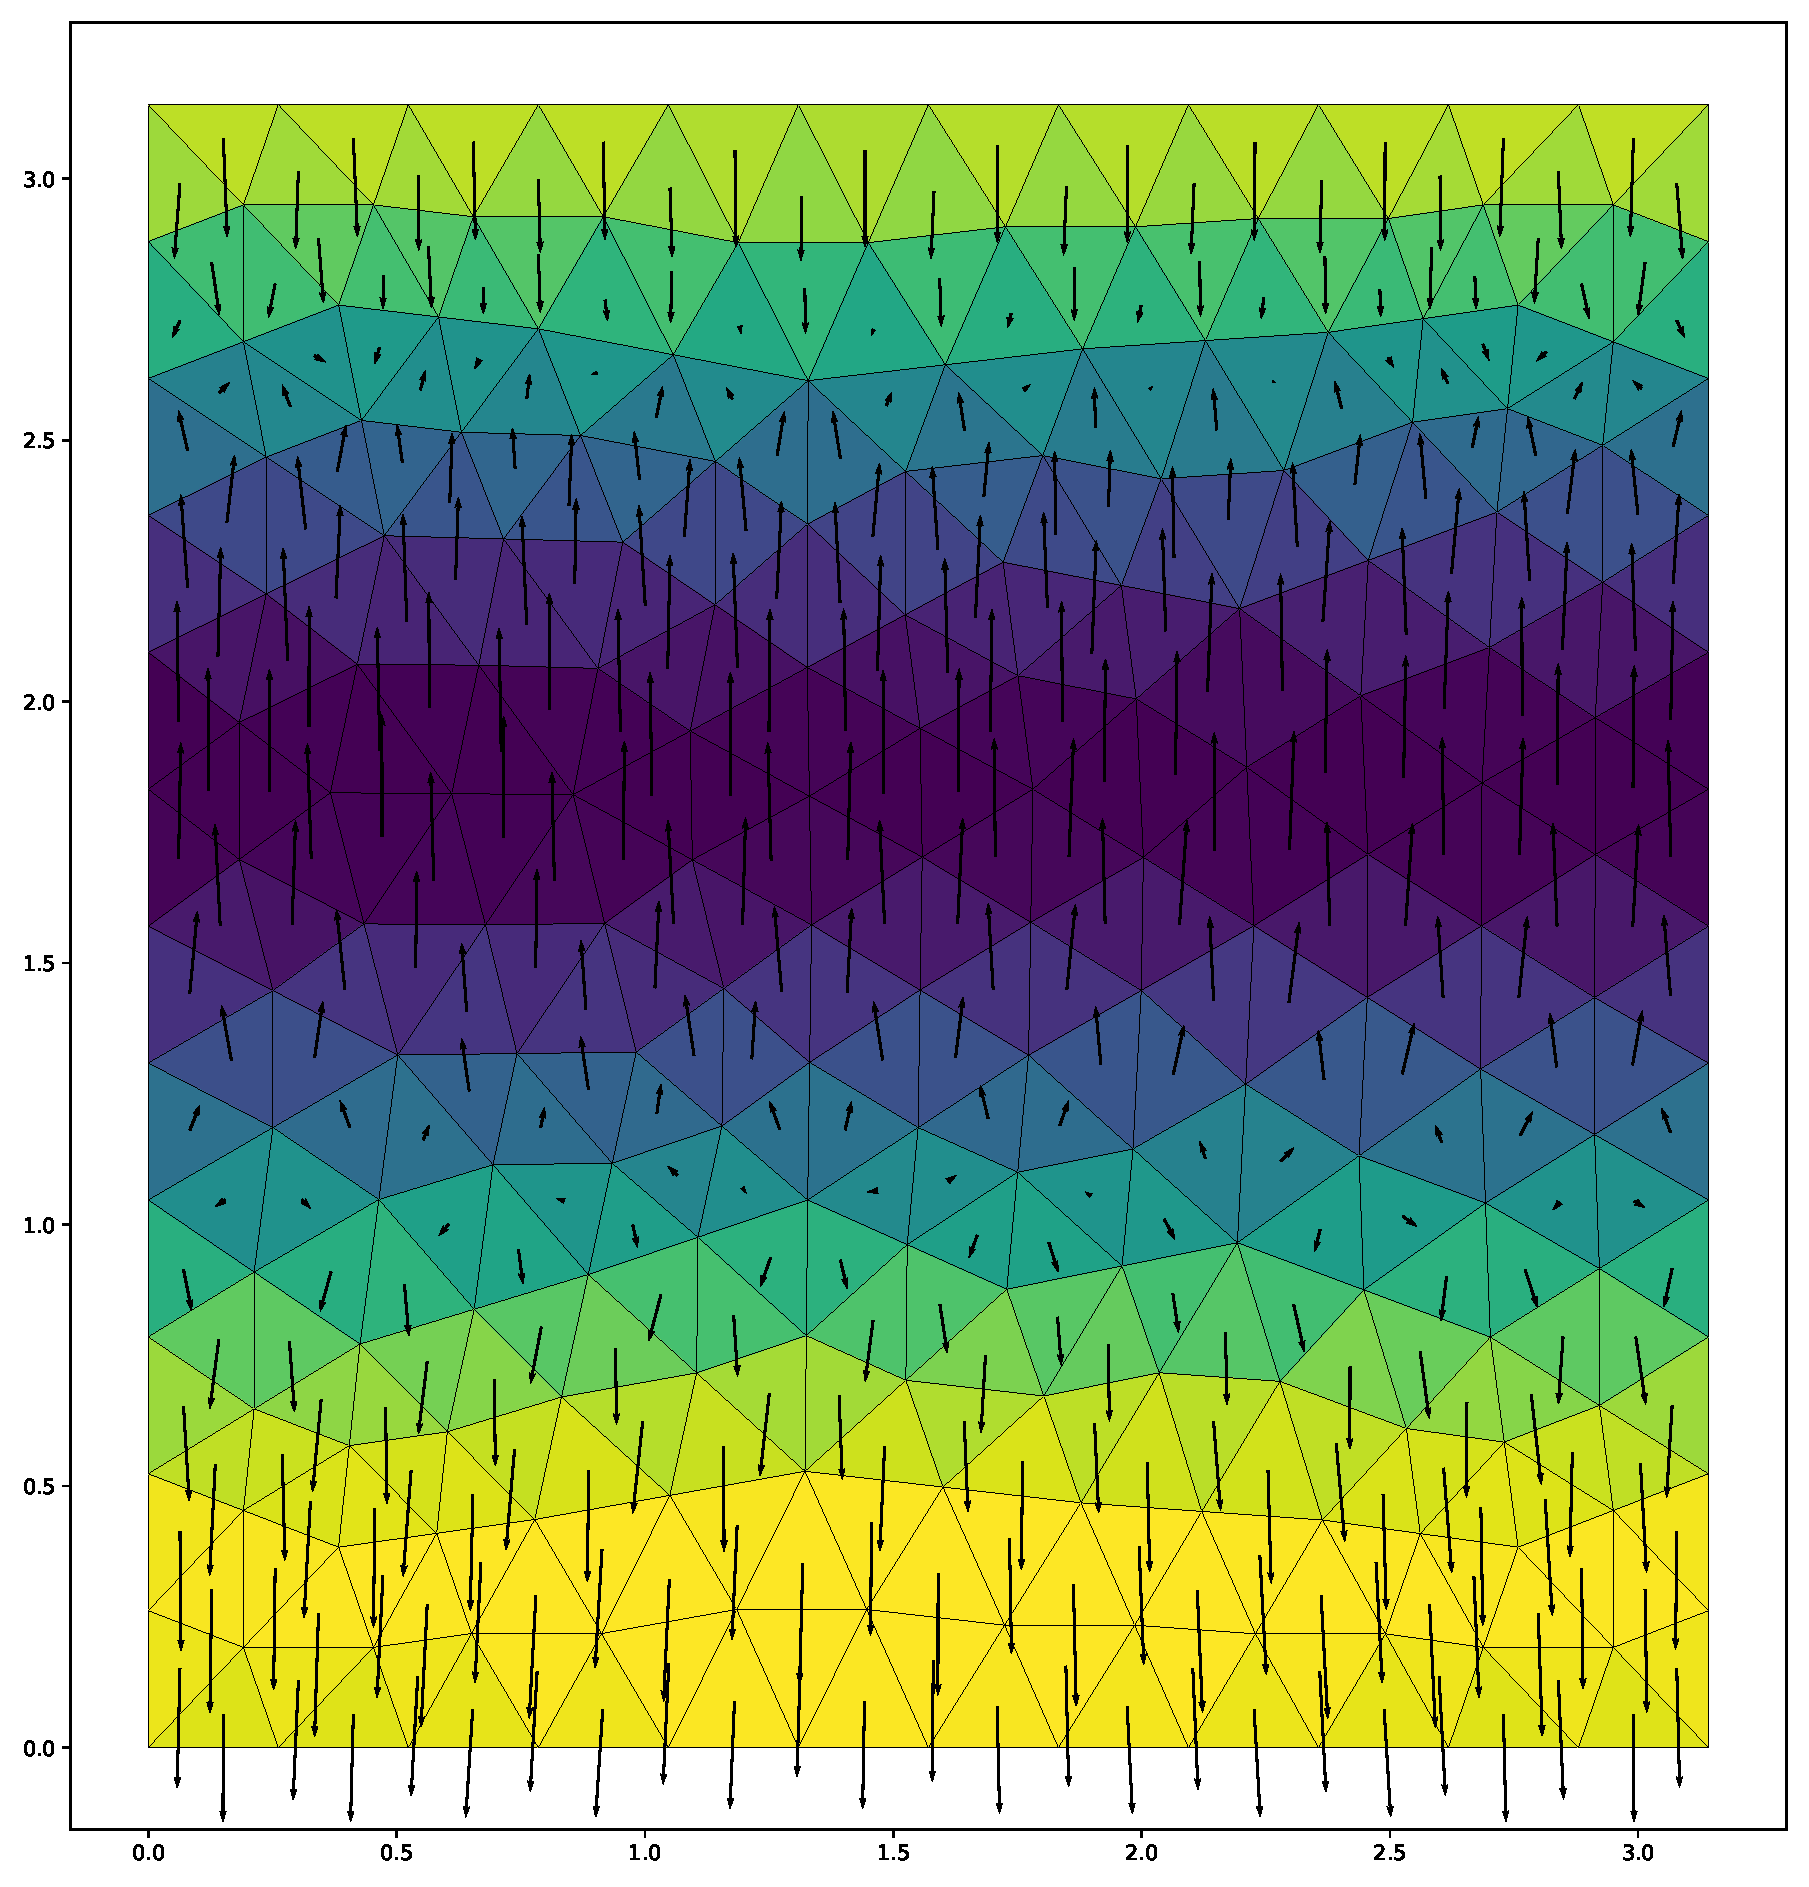
\includegraphics[width=200pt]{thesis/plane_wave.pdf}
  \caption{A plane wave propagating upwards in a square domain.}
  \label{fig:plane_wave}
\end{figure}

It can be shown by substituting the wave \eqref{eq:incident_plane_wave} into 
the second-order acoustic wave equation \eqref{eq:wave2ndOrd}
that it is a solution of the wave equation.
This knowledge is applied to test the accuracy of our simulation.
We apply the wave \eqref{eq:incident_plane_wave}
on the boundary $\Gamma$ as a Dirichlet boundary condition
\begin{equation}\label{eq:plane_wave_boundary_dirichlet}
  q = \star (\nabla \phi_{inc})^{\flat} \quad \text{in } \Gamma \times [0,T]
\end{equation}
(as derived in section \ref{sec:boundary_conditions}),
set the initial conditions to
\begin{align}
  p_0 &= \frac{\partial \phi_{inc}}{\partial t} \Big|_{t=0} \\
  q_0 &= \star (\nabla \phi_{inc})^{\flat} \Big|_{t=0},
\end{align}
and simulate the propagation of the wave in the interior of the domain with DEC.

This simulation is performed several times with progressively reducing
edge lengths on the mesh to investigate the effect of mesh element size on the accuracy.
Error is measured by comparing the simulated values $P$ and $Q$ to the exact cochains
$P_*$ and $Q_*$ obtained by integrating $p = \frac{\partial \phi_{inc}}{\partial t}$
and $q = \star (\nabla \phi_{inc})^{\flat}$ over the corresponding mesh elements.
Because the flux $Q$ is integrated over mesh edges, the error in $Q$ is divided
by edge length to normalize the effect of varying edge lengths on the result.

This experiment is repeated twice, swapping Yee's Hodge star
for the harmonic operators \eqref{eq:harmonic_hodge_1} and \eqref{eq:star_2_harmonic}
derived in section \ref{sec:harmonic_hodge}
and the timestep equations \eqref{eq:timestep_p} and \eqref{eq:timestep_q}
for the exact equivalents \eqref{eq:timestep_p_har} and \eqref{eq:timestep_q_har}
derived in section \ref{sec:exact_timestep}.
The maximum elements of error in pressure and flux
are plotted in figure \ref{fig:accuracy_test_errors}.
The results presented are obtained with the wave parameters
$\omega = 2$ and $\vec{\kappa} = (0,2)$.

\begin{figure}[h]
  \centering
  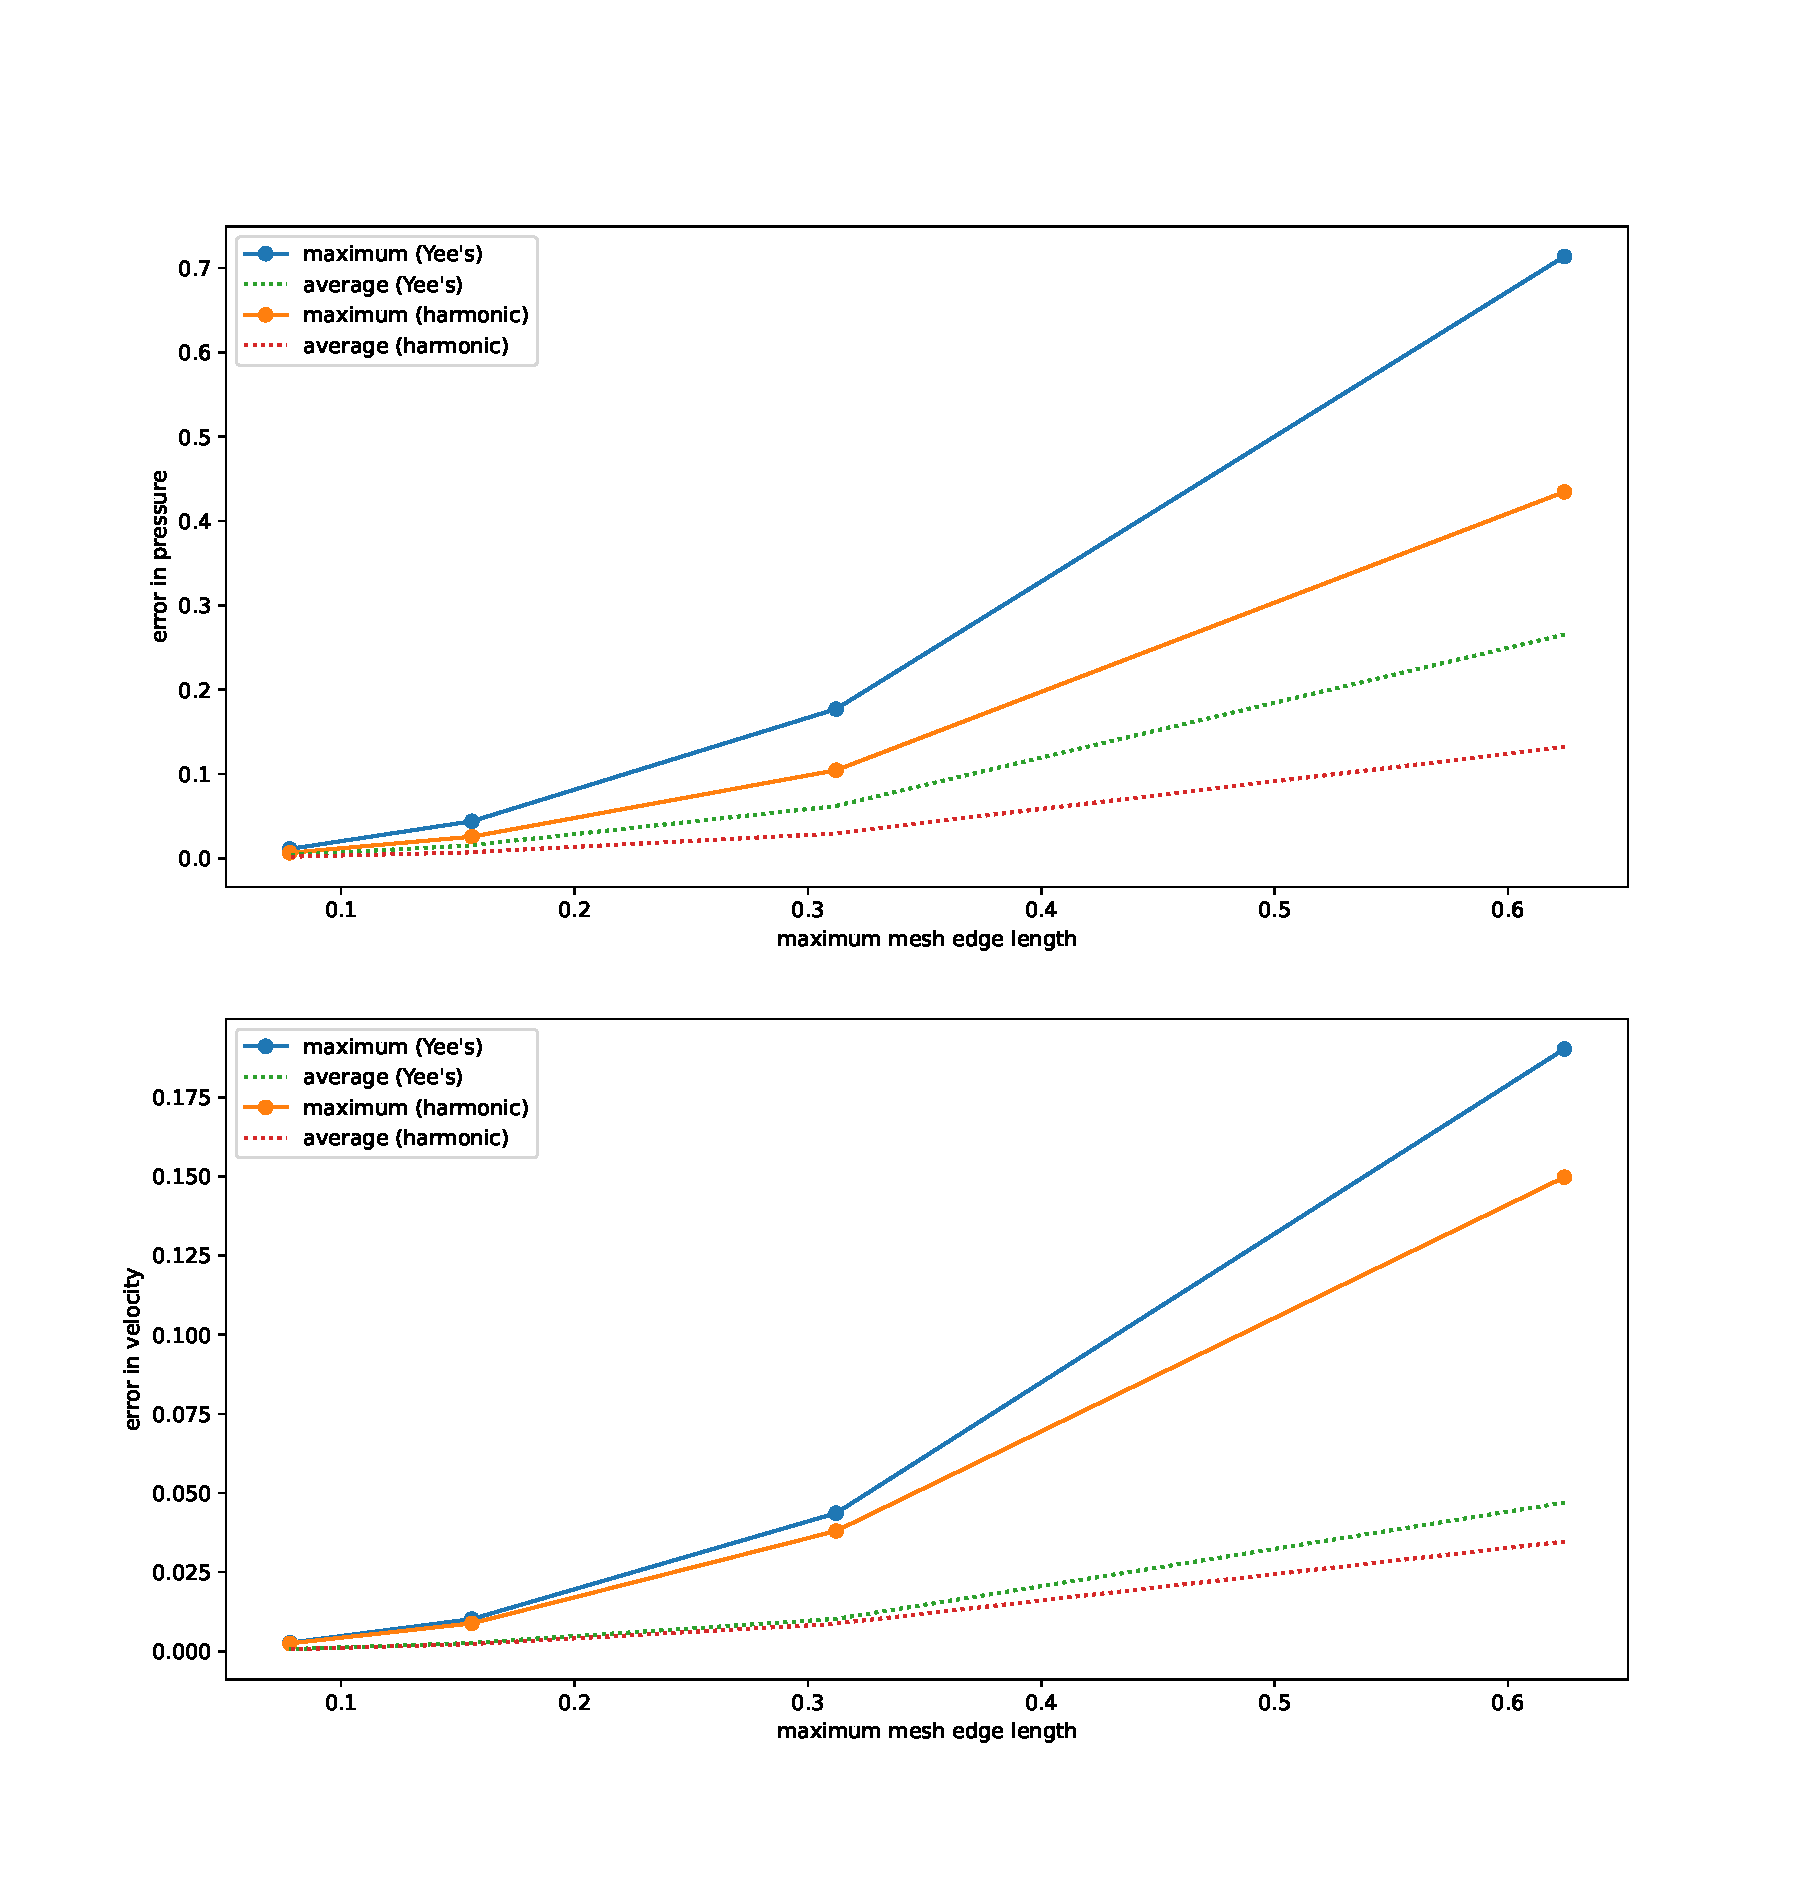
\includegraphics[width=350pt]{thesis/accuracy_test_errors.pdf}
  \caption{Maximum and average error of the simulated plane wave
  in relation to maximum edge length of the mesh.}
  \label{fig:accuracy_test_errors}
\end{figure}

The results show a reduction in error of approximately 40\% in pressure
and varying between 8\% and 20\% in velocity for the harmonic operators.
The harmonic operators add no additional computational cost to the timestepping procedure,
since the Hodge star is still diagonal and the exact timestep coefficient is still a scalar.
Their only cost is a small amount of extra computation beforehand,
which can be performed offline alongside mesh generation if desired.
Thus, they are a highly advantageous addition to the method.

To examine the proportional effects of the harmonic Hodge star and the exact timestep,
note that equations \eqref{eq:timestep_p} and \eqref{eq:timestep_p_har}
only differ by a scalar coefficient.
$\Delta t$ in equation \eqref{eq:timestep_p} is replaced by
$\tau_{ex} = \frac{2}{\omega} \sin \frac{\omega \Delta t}{2}$.
Figure \ref{fig:exact_coef_comparison} plots this value
as a function of the angular velocity $\omega$
with a few selected values of $\Delta t$.
We find that the difference between $\Delta t$ and $\tau_{ex}$
can be significant at high values of $\Delta t$ and $\omega$,
but quickly becomes negligible as $\Delta t$ becomes smaller.

\begin{figure}[h]
  \centering
  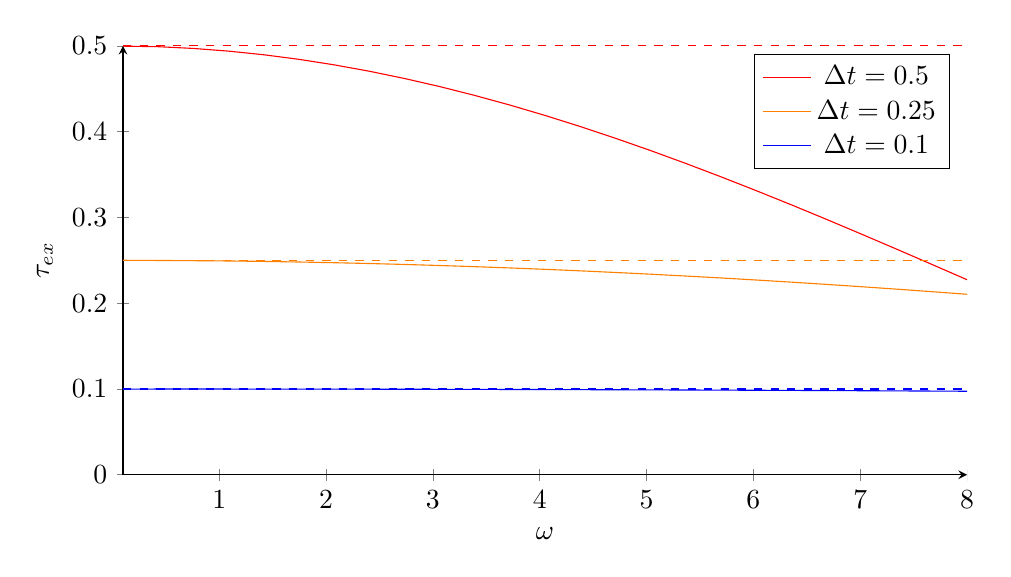
\begin{tikzpicture}
    \begin{axis}[
      domain=0.1:8,
      ymin=0,
      xlabel=$\omega$,
      ylabel=$\tau_{ex}$,
      axis lines=left,
      width=350pt,
      height=200pt,
    ]
      \addplot[color=red]{(2/x)*sin(deg(0.5*x/2))};
      \addlegendentry{$\Delta t = 0.5$}
      \addplot[color=red,dashed,forget plot]{0.5};
      \addplot[color=orange]{(2/x)*sin(deg(0.25*x/2))};
      \addlegendentry{$\Delta t = 0.25$}
      \addplot[color=orange,dashed,forget plot]{0.25};
      \addplot[color=blue]{(2/x)*sin(deg(0.1*x/2))};
      \addlegendentry{$\Delta t = 0.1$}
      \addplot[color=blue,dashed,forget plot]{0.1};
    \end{axis}
  \end{tikzpicture}
  \caption{Effect of angular velocity on the exact timestep coefficient.}
  \label{fig:exact_coef_comparison}
\end{figure}

In our experiments stability generally requires values of $\Delta t$ below $0.1$,
making the effect of the exact timestep minimal.
However, as it requires practically no extra computation,
there is no penalty to implementing it,
and it is potentially beneficial in cases
where stability permits large timesteps.


\section{Scatterer}

Our main experiment uses the entirety of the model defined in chapter \ref{cha:model},
as well as the controllability method covered in chapter \ref{cha:controllability}.
The computation mesh is constructed with two boundaries
as illustrated in figure \ref{fig:scatterer_domain},
with the inner boundary $\Gamma_{sca}$ representing a scattering obstacle
and absorbing outer boundary $\Gamma_{ext}$.
The incident wave, which we set to the plane wave \eqref{eq:plane_wave},
is applied on $\Gamma_{sca}$ as a Dirichlet boundary condition.

The resulting simulation represents the scattered component $\phi_{sca}$
of the total wave $\phi_{inc} + \phi_{sca}$.
We can reconstruct the total wave by adding $\phi_{inc}$ to the result.
By omitting the incident wave from the simulation,
we gain accuracy by eliminating numerical error from the component of the wave
whose exact solution is known.

It is difficult to come up with initial conditions
that fulfill both boundary conditions. 
If we set $p_0 = 0$, $q_0 = 0$, the incident wave is not matched on $\Gamma_{sca}$.
If we set $p_0 = \frac{\partial \phi_{inc}}{\partial t} \Big|_{t=0}$,
$q_0 = \star (\nabla \phi_{inc})^{\flat} \Big|_{t=0}$
like in the previous experiment, the absorbing condition
is not fulfilled on $\Gamma_{ext}$.
This has the effect of a discontinuity on the first timestep of simulation,
which may cause stability issues in particularly unfortunate cases.

To avoid this discontinuity, we use an easing procedure
proposed by \textcite{mur_finite-element_1993}.
Initial conditions are set to $p_0 = 0$, $q_0 = 0$,
and source terms (i.e. values on $\Gamma_{sca}$)
are also initially set to zero.
Source terms are then eased in over a time period $t_{tr}$
by multiplying them by
\begin{equation}\label{eq:mur_transition}
  f_{tr}(t) = (2 - \sin(\frac{\pi}{2} \frac{t}{t_{tr}}))\sin(\frac{\pi}{2} \frac{t}{t_{tr}}).
\end{equation}
This way we get a smooth solution in the entire space and time domain.
To apply this to the controllability method,
we simulate forward in time until $t = t_{tr}$
and use the result as the initial guess for the CG algorithm.

We investigate the convergence of the controllability method
and the asymptotic forward-in-time iteration method
with different scatterer geometries
by measuring the control energy \eqref{eq:control_energy} over time.
Simulating forward one time period $T$ is considered equivalent
to a single step of the controllability method.
We also compare the performance of the Yee's and harmonic operators
in both iteration algorithms.
The scatterer geometries and time-periodic scattered waves
obtained from the controllability method are visualized 
alongside their respective convergence results in figures
\ref{fig:scatterer_square}--\ref{fig:scatterer_diamonds}.
The twelve-pointed star case (fig. \ref{fig:scatterer_star_12})
has wavenumber $\kappa = 2$, while $\kappa = 1$ in the rest of the cases.

\begin{figure}[H]
  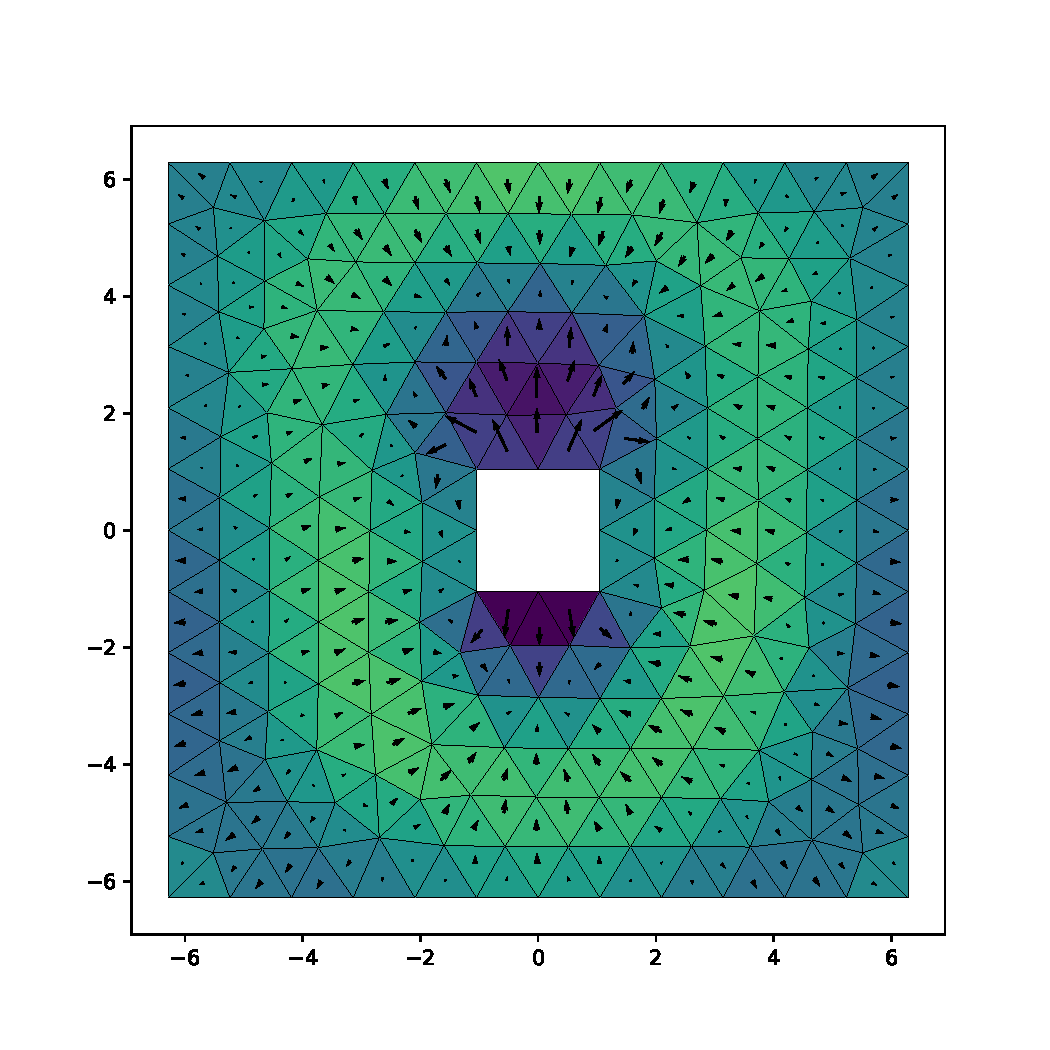
\includegraphics[width=0.49\textwidth]{thesis/scatterer_square_solution.pdf}
  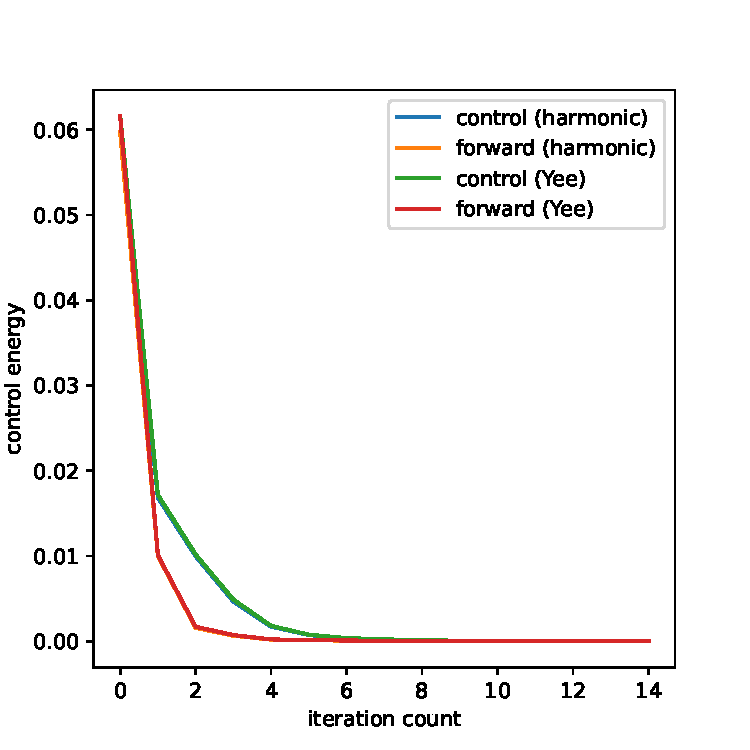
\includegraphics[width=0.49\textwidth]{thesis/scatterer_square_convergence.pdf}
  \caption{Scatterer, case 1: square}
  \label{fig:scatterer_square}
\end{figure}

\begin{figure}[H]
  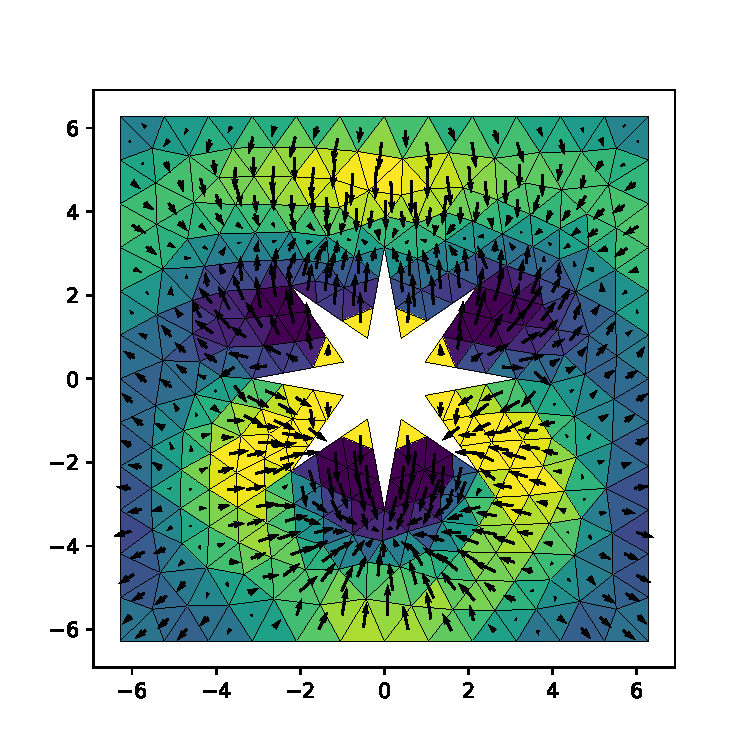
\includegraphics[width=0.49\textwidth]{thesis/scatterer_star_8_solution.pdf}
  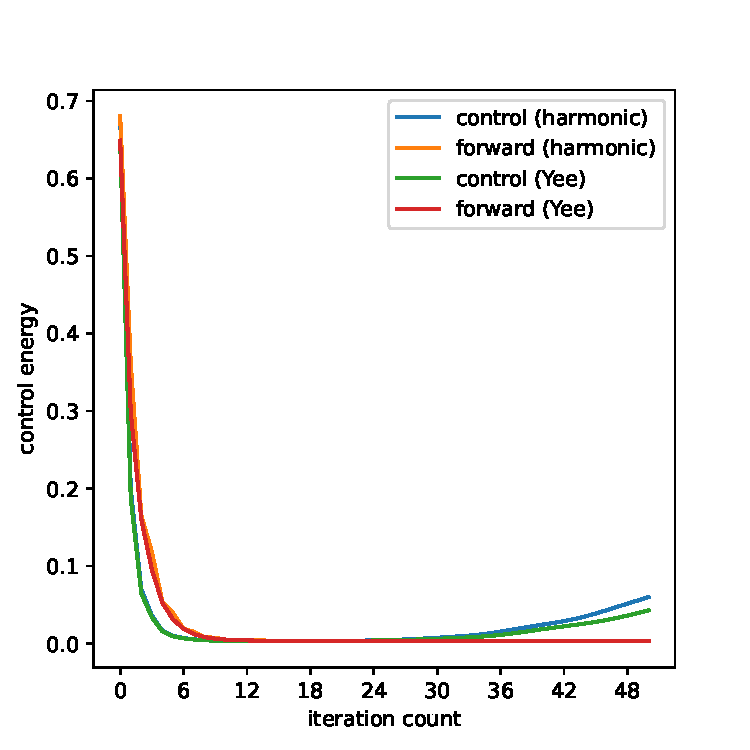
\includegraphics[width=0.49\textwidth]{thesis/scatterer_star_8_convergence.pdf}
  \caption{Scatterer, case 2: eight-pointed star}
  \label{fig:scatterer_star_8}
\end{figure}

\begin{figure}[H]
  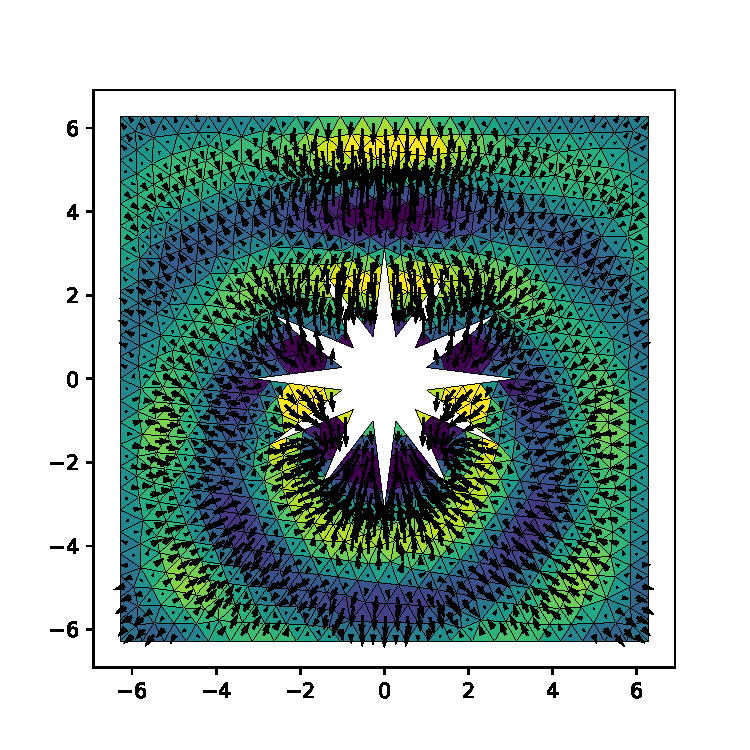
\includegraphics[width=0.49\textwidth]{thesis/scatterer_star_12_solution.pdf}
  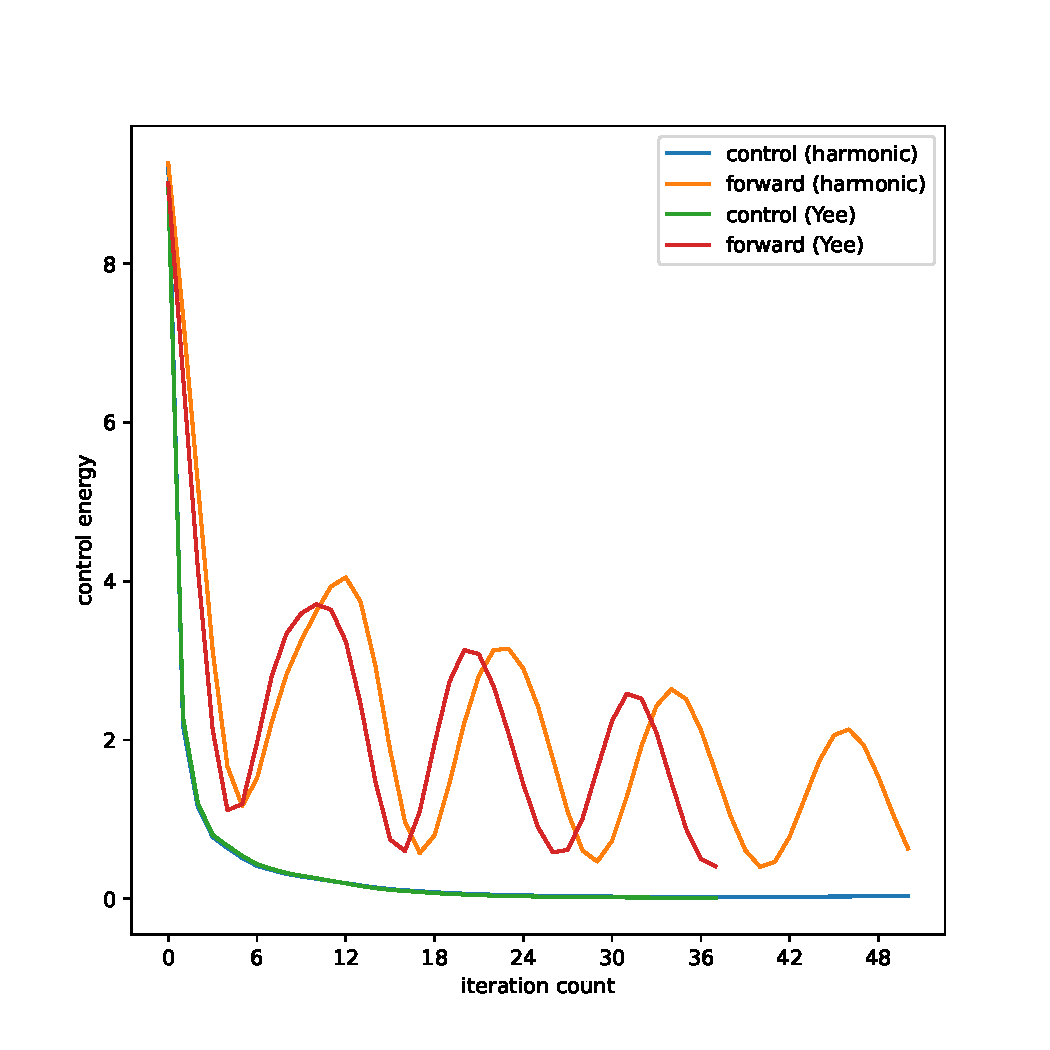
\includegraphics[width=0.49\textwidth]{thesis/scatterer_star_12_convergence.pdf}
  \caption{Scatterer, case 3: twelve-pointed star}
  \label{fig:scatterer_star_12}
\end{figure}

\begin{figure}[H]
  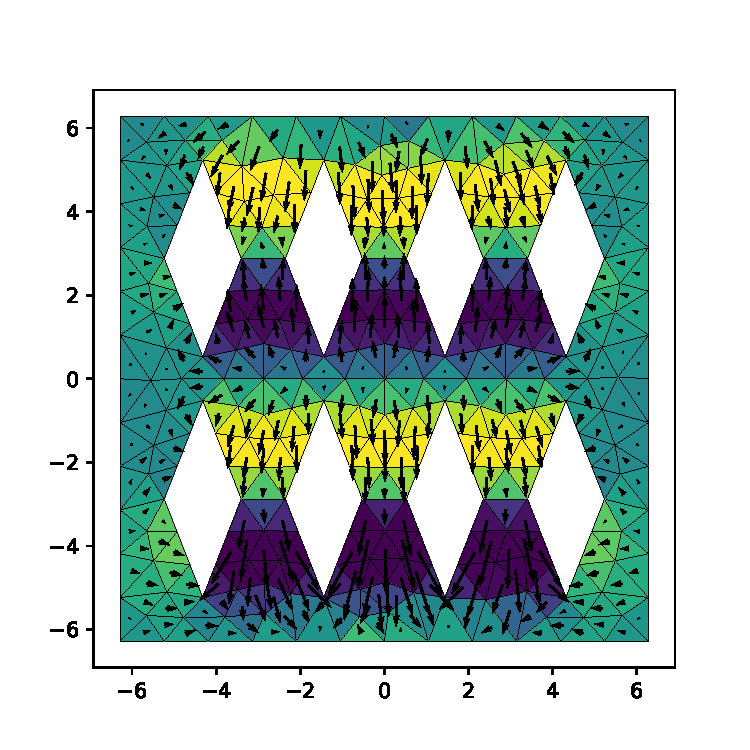
\includegraphics[width=0.49\textwidth]{thesis/scatterer_diamonds_solution.pdf}
  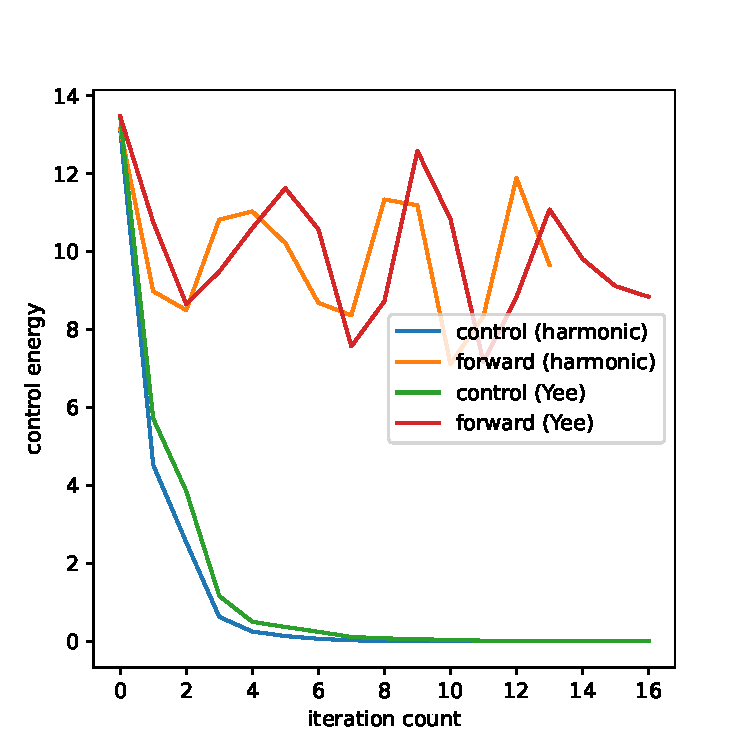
\includegraphics[width=0.49\textwidth]{thesis/scatterer_diamonds_convergence.pdf}
  \caption{Scatterer, case 4: diamonds}
  \label{fig:scatterer_diamonds}
\end{figure}

In the square case we find that the asymptotic iteration method
outperforms the controllability method,
and in the eight-pointed star case it has no strong advantage.
The square is entirely convex, so the scattered wave has no obstacles to slow it down
and reaches the absorbing boundary quickly.
The star is not fully convex, but still allows waves to exit with little obstruction.
In these cases, the optimization approach is not efficient enough
to improve on the rate of convergence.

On the other hand, in the twelve-pointed star and diamonds cases,
where a higher degree of nonconvexity is present
and waves must navigate narrow passages to find the absorbing boundary,
the asymptotic iteration method's performance degrades significantly.
In the diamonds case it fails to reduce energy at all.
The controllability method, on the other hand,
loses little efficiency in these scenarios.

The effects of the harmonic operators on convergence are inconclusive.
They lead to slightly faster convergence in some cases,
but have no advantage in others.
However, it should be noted that the computation
of the control energy \eqref{eq:control_energy}
involves simulating forward in time, which depends on the timestep operators used.
This means that while both operators tend to converge to the same level of energy,
the solutions they converge to are different.
Based on the results of the plane wave experiment,
it can be assumed the harmonic solution is more accurate.

We also note that in the eight-pointed star case, the controllability method's solution
fails to converge to the desired level and the energy begins to increase.
This seems to occur when the computation mesh is of poor quality.
In these cases the mesh produces a high amount of error in the adjoint state solution
when the gradient is close to zero,
causing the CG algorithm's invariants of orthogonal residuals
and $A$-conjugate search directions to be violated.
Unless the mesh quality is poor enough to cause instability,
this does not occur in the asymptotic iteration.

The quality of a mesh can be roughly estimated by investigating
the diagonal values of the Hodge star matrices.
In particular, extremely low values of $\star_1$
arising from short dual edges generate large numerical errors.
Values of $\star_1$ can even become negative
when a dual vertex lies outside its corresponding primal face,
and meshes where this happens were found to give rise to unstable simulations.


\section{Discussion}

The purpose of these experiments was to investigate
the effectiveness of the harmonic time\-step operators
and the controllability method.
The harmonic timestep operators, especially the Hodge star,
offer a notable advantage in accuracy
over Yee's equivalents at a small computational cost,
so their usage can be recommended in all harmonic problems.

The controllability method's results are less clear-cut.
It has a significant advantage in cases with highly nonconvex geometry,
but suffers compared to the asymptotic iteration method
when the geometry is mostly convex.
It also seems to be more sensitive to poor mesh quality
than the asymptotic method.
Its usage should therefore be considered on a case by case basis.

Mesh quality was found to be a major factor in the performance of DEC-based simulations,
and our results likely suffer from the use of a mesh generator
not specifically designed for DEC.
The circumcentric dual mesh is particularly sensitive to narrow triangles
with obtuse angles, which cause the circumcenter to lie outside the triangle.
This produces very small or negative values
in the Hodge star matrix, causing inaccuracy at best and instability at worst.
In future work, the regular crystal meshes of \textcite{rabina_numerical_2014}
and Hodge-optimized triangulations of \textcite{mullen_hot_2011} should be investigated.

While these experiments were performed in $\mathbb{R}^2$,
one of the advantages of DEC is straightforward generalization to higher dimensions.
The main challenges of generalization come from generating the primal mesh
and deriving the harmonic Hodge operators, which needs to be done
for every distinct pair of $k$- and $(n-k)$-cells.
We expect these methods to have similar characteristics and tradeoffs
in higher dimensions.


\chapter{Conclusion}

In this thesis, a numerical method based on discrete exterior calculus (DEC)
and exact controllability was developed
for the purpose of finding time-periodic solutions to acoustic wave scattering problems.
Additionally, a timestepping procedure
and Hodge operator optimized for harmonic problems were investigated.
The harmonic operators were found highly effective,
while the controllability method was only more efficient
than the simpler asymptotic iteration method
in cases with highly nonconvex geometry.
To improve the performance and reliability of the methods,
future development should focus on the quality of the computation mesh,
as the generation methods employed here
are prone to inaccuracies and instabilities.


% suppress overfull hbox errors
\hfuzz=4pt
\printbibliography
\hfuzz=0pt

\end{document}
